% Options for packages loaded elsewhere
\PassOptionsToPackage{unicode}{hyperref}
\PassOptionsToPackage{hyphens}{url}
\PassOptionsToPackage{dvipsnames,svgnames,x11names}{xcolor}
%
\documentclass[
  12pt,
]{article}
\usepackage{amsmath,amssymb}
\usepackage{lmodern}
\usepackage{iftex}
\ifPDFTeX
  \usepackage[T1]{fontenc}
  \usepackage[utf8]{inputenc}
  \usepackage{textcomp} % provide euro and other symbols
\else % if luatex or xetex
  \usepackage{unicode-math}
  \defaultfontfeatures{Scale=MatchLowercase}
  \defaultfontfeatures[\rmfamily]{Ligatures=TeX,Scale=1}
\fi
% Use upquote if available, for straight quotes in verbatim environments
\IfFileExists{upquote.sty}{\usepackage{upquote}}{}
\IfFileExists{microtype.sty}{% use microtype if available
  \usepackage[]{microtype}
  \UseMicrotypeSet[protrusion]{basicmath} % disable protrusion for tt fonts
}{}
\usepackage{xcolor}
\usepackage[margin=1in]{geometry}
\usepackage{longtable,booktabs,array}
\usepackage{calc} % for calculating minipage widths
% Correct order of tables after \paragraph or \subparagraph
\usepackage{etoolbox}
\makeatletter
\patchcmd\longtable{\par}{\if@noskipsec\mbox{}\fi\par}{}{}
\makeatother
% Allow footnotes in longtable head/foot
\IfFileExists{footnotehyper.sty}{\usepackage{footnotehyper}}{\usepackage{footnote}}
\makesavenoteenv{longtable}
\usepackage{graphicx}
\makeatletter
\def\maxwidth{\ifdim\Gin@nat@width>\linewidth\linewidth\else\Gin@nat@width\fi}
\def\maxheight{\ifdim\Gin@nat@height>\textheight\textheight\else\Gin@nat@height\fi}
\makeatother
% Scale images if necessary, so that they will not overflow the page
% margins by default, and it is still possible to overwrite the defaults
% using explicit options in \includegraphics[width, height, ...]{}
\setkeys{Gin}{width=\maxwidth,height=\maxheight,keepaspectratio}
% Set default figure placement to htbp
\makeatletter
\def\fps@figure{htbp}
\makeatother
\setlength{\emergencystretch}{3em} % prevent overfull lines
\providecommand{\tightlist}{%
  \setlength{\itemsep}{0pt}\setlength{\parskip}{0pt}}
\setcounter{secnumdepth}{-\maxdimen} % remove section numbering
\newlength{\cslhangindent}
\setlength{\cslhangindent}{1.5em}
\newlength{\csllabelwidth}
\setlength{\csllabelwidth}{3em}
\newlength{\cslentryspacingunit} % times entry-spacing
\setlength{\cslentryspacingunit}{\parskip}
\newenvironment{CSLReferences}[2] % #1 hanging-ident, #2 entry spacing
 {% don't indent paragraphs
  \setlength{\parindent}{0pt}
  % turn on hanging indent if param 1 is 1
  \ifodd #1
  \let\oldpar\par
  \def\par{\hangindent=\cslhangindent\oldpar}
  \fi
  % set entry spacing
  \setlength{\parskip}{#2\cslentryspacingunit}
 }%
 {}
\usepackage{calc}
\newcommand{\CSLBlock}[1]{#1\hfill\break}
\newcommand{\CSLLeftMargin}[1]{\parbox[t]{\csllabelwidth}{#1}}
\newcommand{\CSLRightInline}[1]{\parbox[t]{\linewidth - \csllabelwidth}{#1}\break}
\newcommand{\CSLIndent}[1]{\hspace{\cslhangindent}#1}
\usepackage{lineno}
\linenumbers
\usepackage{setspace}
\doublespacing
\usepackage{color, soul}
\usepackage{graphicx}
\usepackage{bm}
\usepackage{mathptmx}
\usepackage{array}
\usepackage{caption}
\usepackage{subcaption}
\usepackage[nomarkers]{endfloat}
\usepackage{booktabs}
\usepackage{longtable}
\usepackage{array}
\usepackage{multirow}
\usepackage{wrapfig}
\usepackage{float}
\usepackage{colortbl}
\usepackage{pdflscape}
\usepackage{tabu}
\usepackage{threeparttable}
\usepackage{threeparttablex}
\usepackage[normalem]{ulem}
\usepackage{makecell}
\usepackage{xcolor}
\ifLuaTeX
  \usepackage{selnolig}  % disable illegal ligatures
\fi
\IfFileExists{bookmark.sty}{\usepackage{bookmark}}{\usepackage{hyperref}}
\IfFileExists{xurl.sty}{\usepackage{xurl}}{} % add URL line breaks if available
\urlstyle{same} % disable monospaced font for URLs
\hypersetup{
  colorlinks=true,
  linkcolor={black},
  filecolor={Maroon},
  citecolor={Blue},
  urlcolor={black},
  pdfcreator={LaTeX via pandoc}}

\author{}
\date{\vspace{-2.5em}}

\begin{document}

\renewcommand*{\thefootnote}{\fnsymbol{footnote}}

\begin{centering}
\textbf{\Large{Dynamic spatiotemporal modeling of a habitat defining plant species to support wildlife management at regional scales}}

\textsc{\small{Andrew T. Tredennick\footnote{Current address: Metrum Research Group, Tariffville, Connecticut}\textsuperscript{1}, Adrian P. Monroe\footnote{Corresponding author: \textit{email}, \texttt{amonroe@usgs.gov}}\textsuperscript{2}, Thomas Prebyl\textsuperscript{1}, John Lombardi\textsuperscript{1}, \& Cameron L. Aldridge\textsuperscript{2,3}}}

\textit{\small{\textsuperscript{1}Western EcoSystems Technology, Inc., Laramie, WY}} \\
\textit{\small{\textsuperscript{2}U.S. Geological Survey, Fort Collins Science Center, Fort Collins, CO}} \\
\textit{\small{\textsuperscript{3}Natural Resource Ecology Laboratory and Department of Ecosystem Science and Sustainability, Colorado State University, Fort Collins, CO, in cooperation with U.S. Geological Survey, Fort Collins Science Center, Fort Collins, CO}}

\end{centering}

\renewcommand*{\thefootnote}{\arabic{footnote}}
\setcounter{footnote}{0}

\bigskip{}

\noindent{}\textbf{Open Research Statement}

\noindent{}Code, intermediately derived data, and results are archived on Zenodo (Tredennick et al. 2023a). Projections generated during this study are available as a USGS data release (Tredennick et al. 2023b). All data used in this study are publicly available elsewhere: sagebrush cover data, Rigge et al. (2020); PRISM climate product, \url{http://prism.oregonstate.edu/}; CMIP climate projections, Eyring et al. (2016) accessed with \textbf{epwshiftr} R package (Jia and Chong 2020).

\newpage{}

\hypertarget{abstract}{%
\section{Abstract}\label{abstract}}

Sagebrush (\emph{Artemisia} spp.) ecosystems provide critical habitat for the Greater sage-grouse (\emph{Centrocercus urophasianus}), a species of conservation concern.
Thus, future loss of sagebrush habitat because of land use change and global climate change is of concern.
Here we use a dynamic additive spatio-temporal model to estimate the effects of climate on sagebrush cover dynamics at 32 sage-grouse management areas in Wyoming.
We use the fitted models to quantify the sensitivity of each management area to precipitation and temperature, and to make probabilistic projections of sagebrush cover from present to 2100 under three climate change scenarios.
Global circulation models predict an increase in temperature and no change in precipitation for Wyoming.
Sensitivity to climate varied among management areas but the most common response (70\% of management areas) was a positive effect of temperature on sagebrush performance.
The combination of positive sensitivity to temperature and the predicted increase in temperature under all climate change scenarios resulted in projections of increased sagebrush cover for most management areas.
We characterized management areas as ``optimal'' or ``suboptimal'' based on the percentage of grid cells in each management area with sagebrush cover exceeding a nesting habitat target value.
Only 18\% of management areas are projected to switch from being currently optimal to suboptimal in the future.
Thirty-five percent of management areas are projected to switch from being suboptimal to optimal.
The most common outcome (47\%) was for currently suboptimal management areas to remain suboptimal, even though average cover tended to increase in those areas.
The direct effects of climate change appear to favor sagebrush performance in the future for most sage-grouse core areas in Wyoming.
Our approach is broadly applicable to quantitative climate change assessments where remotely-sensed estimates of habitat-defining vegetation are available.

\emph{Key words:} Artemisia, Centrocercus urophasianus, \emph{climate change, Greater sage-grouse, population model, remote sensing, sagebrush}

\hypertarget{introduction}{%
\section{Introduction}\label{introduction}}

Environmental management and stewardship requires assessing tradeoffs (Walters and Hilborn 1978, Farber et al. 2006).
For example, land managers must consider the long-term effects of climate change and the near-term impacts of ecosystem degradation (e.g., Nepstad et al. 2008).
Because populations, communities, and ecosystems are not static, using the current status of an ecosystem may be insufficient to define protected areas for species (Hannah et al. 2007, Monzón et al. 2011) or to make optimal management decisions (Boettiger et al. 2016).
A better approach is to consider the past, current, and future status of ecosystems.
Doing so requires projections of how an ecosystem might respond to future stressors and conditions (Clark et al. 2001, Dietze et al. 2018).

Wildlife management often requires assessing tradeoffs between the benefits of development and the costs of habitat loss or degradation (McShane et al. 2011).
To assess that tradeoff, managers often identify areas of high and low quality habitat, with low quality habitat preferred for habitat alteration.
But habitat quality is not static and global climate change has the potential to alter the trajectory of an ecosystem.
Some currently high quality habitat (for a particular species) might quickly change if on a range edge while lower quality habitat in the middle of the range might maintain its general structure and function longer (Amburgey et al. 2018).
Habitat on the edge of an ecosystem's range might also improve.
For example, warming temperatures could benefit some plants at the cold edge of their range (Kleinhesselink and Adler 2018).
Thus, climate change adds a new dimension to habitat assessments, where we are not only concerned about the current status of habitat but also what that habitat might look like 30 to 100 years in the future.

Land management in the western United States focuses on several uses and species, but Greater sage-grouse (\emph{Centrocercus urophasianus}, hereafter ``sage-grouse'') has historically driven the conversation in sagebrush dominated ecosystems.
Sage-grouse are a protected species in Canada (Species at Risk Act {[}S.C. 2002, c.~29{]}, \url{https://laws-lois.justice.gc.ca/eng/acts/S-15.3/}) and are listed as ``warranted, but precluded'\,' for listing under the United States Endangered Species Act of 1973 (U.S. Fish and Wildlife Service
{[}USFWS{]} 2010).
A further review of population status and conservation efforts concluded the species did not warrant listing in 2015 (United States Fish and Wildlife Service 2015).
While conservation of sagebrush ecosystems is primarily aimed at keeping sage-grouse off the endangered species list, sagebrush conservation will also benefit other species (Rowland et al. 2006, Smith et al. 2019, Pilliod et al. 2020).
In response to declining sage-grouse populations, the Wyoming Game and Fish Department has delineated 32 sage-grouse core areas, covering approximately 15 million acres of sage-grouse habitat (State of Wyoming 2015).
The stated goal of the Core Area strategy is ``\ldots to minimize future disturbance by co-locating proposed disturbances within area already disturbed or naturally unsuitable'' (State of Wyoming 2015).
Sage-grouse populations are active in all core areas and most maintain stable populations (Edmunds et al. 2018).

Habitat loss and transformation is a major driver of biodiversity loss (Sala et al. 2000, Cardinale et al. 2012, Powers and Jetz 2019), and infrastructure development directly leads to habitat loss and transformation.
Wyoming has ideal conditions for future renewable energy development such as wind (Lloyd et al. 2022), and while wind energy is excluded from sage-grouse core areas, achieving renewable electricity production targets would require expansion beyond disturbed lands (Kiesecker et al. 2011).
This presents a challenge to land management: Should land be prioritized for sage-grouse conservation or renewable energy development?
However, if some areas may become less suitable for sage-grouse due to climate change, those areas might accommodate renewable energy infrastructure without long-term effects on the species.
Considering how climate change impacts whether a sage-grouse core area is or will be ``naturally unsuitable'' clearly falls within the scope of the Core Area strategy.
More broadly, assessing current and future habitat suitability \emph{vis-a-vis} species of concern is useful as we face difficult and inevitable trade-offs between land preservation and land-use to combat climate change.

The sagebrush biome is in peril (Davies et al. 2011, Remington et al. 2021),
but Wyoming is thought to be a stronghold where sagebrush will persist and possibly thrive in the future, especially compared to other parts of its range (Renwick et al. 2018a, Palmquist et al. 2021).
This may partly be due to relatively cooler temperatures in Wyoming (Renwick et al. 2018a) and that Wyoming has largely avoided widespread cheatgrass (\emph{Bromus tectorum} L.) invasion compared to other parts of the sagebrush biome (Pastick et al. 2021).
Cheatgrass invasion, and the subsequent cheatgrass-fire feedback cycle, is the main driver of the loss of sagebrush cover across most of sagebrush's range (Balch et al. 2013).
Because susceptibility to cheatgrass invasion is an indirect effect of climate change (Chambers et al. 2007, Bradley 2009), and because cheatgrass invasion has not been as dramatic in Wyoming, it stands to reason that the direct effects of climate change have important implications in Wyoming.
Indeed, recent modeling suggests that warming temperatures will benefit sagebrush more than cheatgrass at high elevation sites, assuming fire is limited (Palmquist et al. 2021).
Therefore, this paper focuses on modeling the direct effects of climate on sagebrush cover change.

Here we describe a computationally efficient Bayesian spatiotemporal modeling approach for making probabilistic projections of sagebrush cover dynamics under the direct effects of climate change in Wyoming, USA using remotely sensed cover estimates.
A key feature of our approach is using the probabilistic projections to evaluate specific management targets for sagebrush cover in sage-grouse core areas, with implications for other sagebrush-dependent wildlife (Remington et al. 2021).
Specifically, our goals are to: i) quantify the sensitivity of sagebrush percent cover in sage-grouse core areas to temperature and precipitation, ii) use the fitted models to project sagebrush percent cover into this future under climate change scenarios, and iii) evaluate the projections relative to sagebrush cover targets and current sage-grouse status in each core area.
Our approach is applicable to diverse situations where clear management targets exist and spatiotemporal data are available to train probabilistic models.

\hypertarget{materials-and-methods}{%
\section{Materials and Methods}\label{materials-and-methods}}

\hypertarget{data}{%
\subsection{Data}\label{data}}

\hypertarget{remotely-sensed-time-series}{%
\subsubsection{Remotely-sensed time series}\label{remotely-sensed-time-series}}

We used the Rangeland Condition, Monitoring, Assessment, and Projection (RCMAP) data product from the National Land Cover Database (NLCD), a product of the Multi-Resolution Land Characteristics Consortium (Rigge et al. 2020).
We downloaded the ``NLCD BIT Sagebrush Fractional Component'' estimates for each year from 1985 to 2018, subset the data to the Wyoming sage-grouse core areas, and then resampled the data up to 100-meter resolution using bilinear interpolation to aggregate cover across 30-meter grid cells.
We resampled the data to make the analysis computationally tractable: decreasing the spatial resolution resulted in fewer cells of data per year and thus reduced the total size of the observed data.
Time series of cover are shown in Fig. \ref{fig:data}.
There are no data for 2012, which we handled naively by letting 2011 be the ``lag cover year'' for 2013.
The BIT products are estimates with associated error (Rigge et al. 2020), which we ignore in this analysis.
Assuming errors are not related to time or space, the impact of including error would likely increase the error of estimates in the model described below.

\begin{figure}
\centering
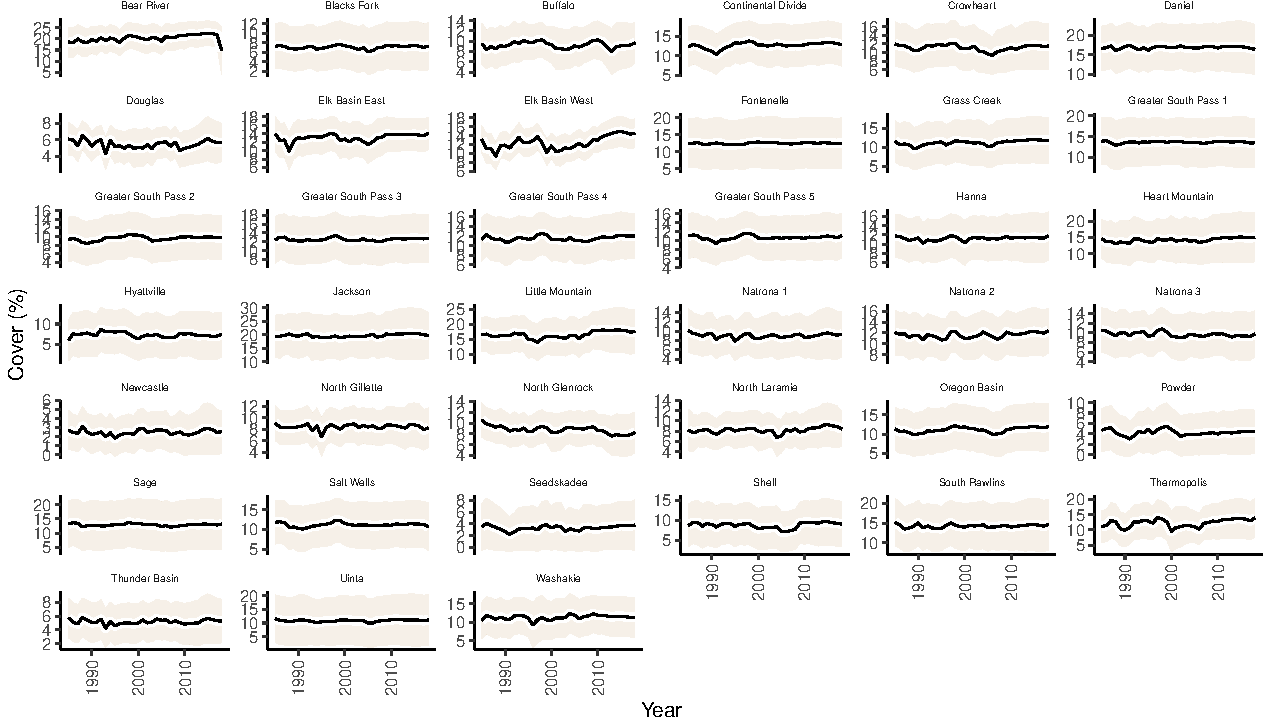
\includegraphics{sageCastManuscript_files/figure-latex/data-1.pdf}
\caption{\label{fig:data}Observed time series of percent cover for each sage-grouse core area in Wyoming, USA from the NLCD BIT Sagebrush Fractional Component product. Line shows mean cover in each year across all cells (pixels). The shaded region shows the mean plus/minus the standard deviation across all cells (pixels) in each year. Note that the y-axis changes across panels.}
\end{figure}

\hypertarget{climate-covariates}{%
\subsubsection{Climate covariates}\label{climate-covariates}}

We downloaded historical climate estimates from PRISM (\url{http://prism.oregonstate.edu/}), with spatial extents that matched the sage-grouse core areas.
PRISM data were resampled to 100-m resolution using bilinear interpolation to match the BIT data.
From these estimates, we calculated two climate covariates: 1) average spring-through-summer temperature and 2) average spring-through-summer precipitation.
We defined spring-through-summer as March 1 through August 31 for each year.
We decided on the two covariates based on our previous work (Tredennick et al. 2016) and more recent work by Kleinhesselink and Adler (2018).
Previous modeling of sagebrush dynamics in Wyoming and across the sagebrush range used ``lagged covariates'' like precipitation in the year prior to an observed transition.
We do not use lagged covariates here because exploratory work indicates that lagged covariates result in correlated and confounded parameter estimates (Kleinhesselink written pers. comm., 2021).

The choice to use two simple covariates is motivated by biology, modeling constraints, and the desire to avoid spurious, difficult-to-explain effects.
First, as mentioned above, average spring-through-summer precipitation and temperature have been identified as important covariates in previous work (Tredennick et al. 2016, Kleinhesselink and Adler 2018).
These two covariates also have the advantage of being directly tied to the limits of sagebrush performance in terms of cold, moist versus warm, dry sites (Palmquist et al. 2021).
Second, the models we fit are computationally intensive due to the large size of each core area and the number of core areas we modeled.
Avoiding variable selection reduces some computational constraints.
We also needed to use covariates that could be easily extracted and computed from GCM output for future projections.
Last, given the number of core areas we modeled, the use of many covariates could increase the chance of detecting spurious effects, which we sought to avoid.

\hypertarget{climate-projections}{%
\subsubsection{Climate projections}\label{climate-projections}}

We used climate projections from Global Circulation Models (GCMs) that contributed to the CMIP6 project (Eyring et al. 2016).
Groups that contributed to CMIP6 provided output from several experimental conditions.
We used three common experimental conditions for generating future projections under different shared socio-economic pathways (SSPs): ssp126 (low future carbon emissions), ssp245 (intermediate future carbon emissions), and ssp585 (high future carbon emissions) (see Eyring et al. (2016) for more details).
ssp126 is a version the RCP2.6 scenario and assumes that radiative forcing reaches 2.6 W/m\(^2\) in 2100.
ssp245 is a version of the RCP4.5 scenario and assumes that radiative forcing reaches 4.5 W/m\(^2\) in 2100.
ssp585 is a version of the RCP8.5 scneario and assumes that radiative forcing reaches 8.5 W/m\(^2\) in 2100.
GCM ouputs were downloaded from Lawrence Livermore National Library archives of CMIP6 model simulations and projections.
We used the \texttt{esfg\_query} function from the \textbf{epwshiftr} R package (Jia and Chong 2020) to query the database and download the data.
GCMs had to include historic, ssp126, ssp245, and ssp585 scenarios for inclusion.
In total, we compiled future climate projections from 18 GCMs.
We applied a bias correction to the GCM values by shifting the means of GCM projections in reference to PRISM data from the historical time period.

GCM projections vary in their accuracy depending on location.
Therefore, we weighted each of the GCMs by their ability to reproduce observed data (Rupp et al. 2013).
To evaluate each GCM we compared historical projections (1985 - 2018) from each GCM to PRISM data for the same time span and geographic area.
For each year we resampled the historic GCM raster data to match the spatial resolution of the PRISM data and extracted values for the two climate variables (average spring-through-summer temperature and average spring-through-summer precipitation) for each sage-grouse core area, then calculated the mean climate variable value across all core areas.

Following Rupp et al. (2013), we calculated the relative error (\(E^*\)) across the entire time span for both climate variables and for each GCM as

\begin{equation}
E_{i,j}^* = \frac{E_{i,j} - \min\limits_{i}(E_{j})}{\max\limits_{i}(E_{j}) - \min\limits_i(E_{j})}
\end{equation}

\noindent{}where \(i\) indexes the variable (temperature or precipitation) and \(j\) indexes the GCM.
\(E_{i,j}\) is the mean absolute error, calculated as \(E_{i,j} = \left(\sum_{k=1}^K|x_{i,j,k} - z_{i,j,k}|\right)/{K}\), where \(x\) is the observed value from PRISM and \(z\) is the value from the GCM and \(k\) indexes the observation (an annual mean value for a particular year), and \(K\) is the total number of observations.
Last, we averaged the \(E^*\) values across the two variables (temperature and precipitation) to arrive at a single relative error value for each of the \(J\) GCMs: \(E_{j}^* = \left(\sum_{i=1}^N E_{i,j}^* \right) / N\), where \(N = 2\) is the total number of variables.
The resulting relative errors for each GCM were used as weights (\(w_j = 1 - E_j^*\)) when making projections of sagebrush dynamics forced by the GCM output.
Specifically, the projected time series of weather we used under each scenario is the weighted average of all GCMs, with \(w_j\) being the weight for each GCM \emph{j}.
For simulating projections, GCM data were resampled from 100-km resolution to 1-km resolution, cropped to each core area extent, and then the average covariate value across 1-km grid cells within each core area was calculated.
This means that climate covariates for projections did not vary across space within each core area, only over time.

\hypertarget{model}{%
\subsection{Model}\label{model}}

\hypertarget{dynamic-additive-spatio-temporal-model-for-sagebrush-cover}{%
\subsubsection{Dynamic additive spatio-temporal model for sagebrush cover}\label{dynamic-additive-spatio-temporal-model-for-sagebrush-cover}}

We used a descriptive, dynamic model of sagebrush cover, building on our previous work (Tredennick et al. 2016) and animal population modeling described by Conn et al. (2015).
Models were fit to each core area independently.
For each core area, our model represents the observed sagebrush cover in cell \emph{i} of year \emph{t} (\(y_{i,t}\)) as arising from a Poisson process with rate \(\text{exp}(\mu_{i,t})\):

\begin{equation}
y_{i,t} \sim \text{Poisson}(\text{exp}(\mu_{i,t})).
\end{equation}

\noindent{}The deterministic process model follows the log-transformed version of a Gompertz population growth model, representing \(\mu_{i,t}\) as

\begin{equation}
\label{eq:regression}
\mu_{i,t} = \bm{\beta} x_{i,t} + \gamma_{t} + w_{i}
\end{equation}

\noindent{}where \(\bm{\beta}\) is a vector of regression coefficients, \(x_{i,t}\) is a vector of covariates for cell \emph{i} at time \emph{t}, \(\gamma_{t}\) is a temporal random effect, and \(w_i\) is a spatial offset for each cell \emph{i}.
The covariate vector \(x_{i,t}\) is one row of the design matrix \(\textbf{X}\), which includes a column of 1s for the intercept, a column of logged lag cover (\(\text{log}(y_{t-1})\)) values, a column for the precipitation covariate, and a column for the temperature covariate.
\(\textbf{X}\) is a \(n \times p\) matrix and each row represents a single observation, indexed by time (\(t\), year of observation) and cell (\(i\), spatial location).
We added a small offset (0.0001) to all one-year lagged observed percent cover values that occur in the design matrix \(\textbf{X}\) before logging those values so that 0 cover values could be included easily.
There were very few instances of 0 cover, so this work-around likely had small, if any, influence on the results.

In previous work we estimated the spatial offset using kernel convolution and dimension reduction (Tredennick et al. 2016).
Estimating the spatial offset is not strictly necessary because the data represent a full sample of the spatial domain.
Here we use an empirical approach to calculate the spatial offset because it substantially reduces computational time and results in a better representation of the spatial variance.
We calculated the spatial offset for each grid cell as the difference between the log of the focal mean of a cell over time and the log of mean cover across each complete core area over time. More specifically, we calculated the spatial offset \(w_i\) for each cell \emph{i} in a core area as

\begin{equation}
w_{i} = {\text{log}(\bar{f}_{i}) - \text{log}(\bar{y})},
\end{equation}

\noindent{}where \(\bar{y}\) is the mean cover across all years and cells within the core area and \(\bar{f}_{i}\) is the weighted focal mean of all surrounding cells within a radius \emph{r},

\begin{equation}
\bar{f}_{i} = \frac{1}{n} \sum_{j=1}^{n}x_{j} \times k_{j},
\end{equation}

\noindent{}with weights, \(k_{j}\), defined using an exponential decay function,

\begin{equation}
k_{j} = \text{exp}\left( \frac{-d_{j} }{\left(r\times\frac{1}{3} \right)} \right),
\end{equation}

\noindent{}where \(d_j\) is the distance in meters from cell \emph{j} to focal cell \emph{i} and \emph{n} is the total number of cells within the radius \emph{r} of the focal cell.
We defined \emph{r} as the maximum range of spatial dependence in residuals from a simple generalized linear model (GLM) fit without climate covariates for each core area (Tredennick et al. 2016).
The \texttt{focal} function from the \textbf{raster} package (Hijmans et al. 2023) in R cannot accommodate missing values when calculating a focal mean with custom weights.
We pre-filled any cells with missing cover values using a focal mean with equal weight for all cells within the analysis radius \emph{r}.
After calculating \(\bar{f}_{i}\), all cells that originally had missing cover values were re-set to \texttt{NA} before calculating the final spatial offset value \(w_i\).
Missing cover values corresponded to masked areas not defined as ``sagebrush'' habitat in the RCMAP products.

The full Bayesian posterior distribution of the dynamic-additive spatiotemporal model is:

\begin{align}
\left[\bm{\beta}, \bm{\gamma}, \sigma_{\gamma} | \textbf{y}, \textbf{X}, \textbf{w} \right] &\propto  \prod^T_{t=1} \prod^N_{i=1} \left[ y_{i,t}| \bm{\beta}, \gamma_t, w_i \right] \nonumber \\
&\times \left[ \gamma_t | \sigma_{\gamma} \right] \nonumber  \\
&\times \left[\bm{\beta}  \right] \left[ \sigma_{\gamma}\right].
\end{align}

An attractive feature of the Gompertz population model in log space (Eq. \ref{eq:regression}) is that equilibrium abundance is defined as: \(\mu' = \beta_1 / \left(1 - \beta_2 \right)\) (Ives et al. 2003, Kleinhesselink and Adler 2018).
Note that this definition holds when the random effects are centered on 0 and when the covariates are scaled and centered on 0.
Both of these conditions hold in our model.
We use equilibrium abundance (cover, in our case) as a starting point for sensitivity analyses.
For example, equilibrium cover across all cells in a core area is \(\overline{y}' = \text{exp}(\mu')\).
Equilibrium cover for a particular cell (\emph{i}) is \(y_i' = \text{exp}(\mu' + w_i)\).
Equilibrium cover for a particular cell (\emph{i}) under a climate scenario where the future climate is 1 standard deviation greater than current climate is \(y_i' = \text{exp}\left(\mu' + w_i + (1\times\beta_3) + (1\times\beta_4) \right)\) (Kleinhesselink and Adler 2018).
Projections of future cover were initialized with observed cover in 2018.

We used results from Tredennick et al. (2016) to define informative prior distributions for the intercept (\(\beta_1\)) and density-dependence (\(\beta_2\)) regression parameters in Eq. \ref{eq:regression} (Table \ref{tab:priors}).
Vague prior distributions were assigned to all other parameters (Table \ref{tab:priors}).

\begin{table}[tbp]
\caption{\label{tab:priors}Prior distributions for the dynamic-additive spatiotemporal regression model of sagebrush cover. Standard deviations from Tredennick et al. (2016) were replaced with 1 for the intercept and density-dependence terms to generate a slightly more skeptical prior.}
\small
\begin{tabular}{p{0.1\linewidth}p{0.35\linewidth}p{0.2\linewidth}p{0.2\linewidth}}
\hline
Parameter & Definition & Distribution & Source \\ \hline
$\beta_1$ & intercept  & Normal(0.73, 1) & Tredennick et al. (2016) \\
$\beta_2$ & density-dependence & Normal(0.72, 1) & Tredennick et al. (2016) \\
$\beta_{3\&4}$ & effects of precipitation ($\beta_3$) and temperature ($\beta_4$) & Normal(0, 5) & --  \\ 
$\bm{\gamma}$ & temporal random effects & Normal(0, $\sigma_{\gamma}$) & -- \\
$\sigma_{\gamma}$ & standard deviation of temporal random effects & Cauchy(0, 2.5) & -- \\ \hline
\end{tabular}
\end{table}

\hypertarget{model-fitting-and-evaluation}{%
\subsubsection{Model fitting and evaluation}\label{model-fitting-and-evaluation}}

We used Hamiltonian Monte Carlo (HMC) to approximate the posterior distributions of all unknown parameters.
Specifically, we used the Stan software (Stan Development Team 2020) to implement the HMC Markov chain Monte Carlo (MCMC) algorithm, using the rstan package (Guo et al. 2020) to connect Stan to R.
We ran three chains of 1,000 iterations after a burn-in of 1,000 iterations.
Convergence of the MCMC chains was assessed visually with traceplots and by ensuring that the 95\% upper credible interval of scale reduction factors (\(\hat{R}\)) were less than 1.1 (Gelman and Rubin 1992, Gelman and Hill 2006).
Convergence diagnostics for the intercept (\(\beta_1\)) and the temporal random effects (\(\gamma_t\)) were computed after applying ``post-sweeping'' to address mixing and convergence problems associated with weak identifiability (Ogle and Barber 2020).

We used a subset of the data to fit the model.
We did this to make estimation via MCMC possible in a reasonable time frame.
We extracted a spatially balanced 5\% sample of grid cells from each core area to use for model fitting.
We used the function \texttt{bas.polygon} from the \textbf{SDraw} R package (McDonald et al. 2020) to sample the grid cells for model fitting.
Some core areas (e.g., Greater South Pass) were divided into smaller subsets that were fitted independently due to memory constraints.
Core areas that were divided are indicated by having a number next to their name or abbreviation (e.g., Greater South Pass 1, Greater South Pass 2, etc.).
Note that the spatial offsets for each grid cell \emph{i} (\(w_i\)) were calculated for the entire spatial domain and then we extracted the 5\% sample of all relevant information: cover, lag cover, climate covariates, and the spatial effects for each selected grid cell.

We used posterior predictive checks to calculate Bayesian \emph{P} values assessing the lack-of-fit between the model and the data (Hobbs and Hooten 2015, Conn et al. 2018).
We simulated cover data for each cell and year (\(y^{\text{new}}_{i,t}\)) from the model at each MCMC iteration and used a chi-square statistic to compare the data (both original and ``new'' data) to the expected values from the deterministic regression model.
The test statistics were then summed over time and space separately, yielding test statistics for each cell over years for both the new and original datasets,

\begin{equation}
\tau^{\text{new}}_i = \sum^Y_{t=1} \frac{\left(y^{\text{new}}_{i,t} - \mu_{i,t}\right)^2}{\mu_{i,t}}    
\end{equation}

\noindent{}and

\begin{equation}
\tau_i = \sum^Y_{t=1} \frac{\left(y_{i,t} - \mu_{i,t}\right)^2}{\mu_{i,t}},    
\end{equation}

\noindent{}and for each year over cells for both the original and new datasets,

\begin{equation}
\tau^{\text{new}}_t = \sum^S_{i=1} \frac{\left(y^{\text{new}}_{i,t} - \mu_{i,t}\right)^2}{\mu_{i,t}}    
\end{equation}

\noindent{}and,

\begin{equation}
\tau_t = \sum^S_{i=1} \frac{\left(y_{i,t} - \mu_{i,t}\right)^2}{\mu_{i,t}}.    
\end{equation}

\noindent{}We then computed Bayesian p-values as the proportion of the total number of MCMC iterations for which \(\tau^{\text{new}} > \tau\) for each cell or year.
Lastly, we averaged the Bayesian p-values over years and cells to compute two final p-values to evaluate lack-of-fit: one for lack-of-fit over the spatial dimension (\(P_B^{\text{space}}\), averaged over years) and one for lack-of-fit over the temporal dimension (\(P_B^{\text{time}}\), averaged over cells).
Posterior predictive checks were done using a new spatially balance sample of the data (i.e., a different sample than used to fit the model).

All computations were done in R (R Core Team 2020).
We bundled the computer code needed to format data, fit the model, evaluate the model, and project the model forward in an R package called \textbf{sageCastR} (\url{https://github.com/WEST-Inc/sageCastR}, archived on Zenodo Tredennick et al. (2023a)).
Note that the R package is not a generalizable piece of software; it is a code bundle for this particular project.
We also note that fitting the models required a high memory machine and parallel processing.
Interested users can modify the code for future research.

\hypertarget{model-projections}{%
\subsubsection{Model projections}\label{model-projections}}

We made projections of sagebrush cover in each core area under each of the three climate change scenarios (ssp126, ssp245, and ssp585).
Initial conditions were defined as the last year of BIT cover estimates for each core area.
Climate covariates for each year were calculated as the weighted averages across the GCMs.
The weighted averages for the precipiation and temperature covariates were then scaled using the mean and standard deviation for each covariate from the model fitting stage.
This was done independently for each core area and was necessary because we used Z-score transformed covariates for model fitting.
We projected sagebrush cover to the year 2100, using 50 random MCMC parameter sets to approximate the posterior predictive distribution (Hobbs and Hooten 2015).
We used 50 posterior parameter sets instead of the full posterior distribution (3000 MCMC parameter sets) to decrease computation time and data storage.

We also used a colonization model when projecting the model forward to avoid local extinction in grid cells.
We fit a bimonial regression model for each core area to estimate the probability of a grid cell with zero percent cover in year \emph{t} transitioning to non-zero cover in year \emph{t+1} (Tredennick et al. 2016).
This probability was used in the dynamic projections whenever a grid cell had zero cover to simulate whether the grid cell would stay at zero or increase to non-zero cover.
We calculated the average cover in cells that transitioned from zero cover to non-zero cover for each core area.
Those values were used in the simulation model as the cover assigned to cells that were simulated to transition from zero cover to non-zero cover.
Projections generated during this study are available as a USGS data release (Tredennick et al. 2023b).

Our main goal was to evaluate future cover projections relative to specific management targets.
We defined two management targets: 1) the percent cover needed at 100-meter resolution to maintain sage-grouse nesting habitat and 2) the percent cover needed at 100-meter rosultion to maintain sage-grouse summer habitat.
We used the 1985-2018 sagebrush cover rasters (resampled to 100 m resolution) to determine the 95\% quantile of the time series for each pixel.
This quantile should indicate potential sagebrush cover at each pixel while reducing the influence of temporal annomalies.
Then, we divided Wyoming into three regions (southwest, central, and northeast) and determined the median value across all 95\% quantiles that intersected either nesting or summer sage-grouse habitat, by region (Fedy et al. 2014).
These provided threshold values for nesting and summer habitat that were region-specific yet consistent with thresholds recommended by the Sage-grouse Habitat Assessment Framework: 15-25\% cover for nesting and 10-25\% cover for summer (Stiver et al. 2015).
The threshold values we calculated are provided in the online supporting information (Appendix S1: Table S81).

Based on Fedy et al. (2014), we set our lanscape level management goal to be 50\% of grid cells in a core area meeting or exceeding the nesting target percent cover value.
We defined core areas as ``optimal'' or ``suboptimal'' for sage-grouse based on this management goal: optimal = 50\% of grid cells meeting or exceeding the nesting target, suboptimal = 50\% of grid cells below the nesting target.
We futher categorized core areas into four groups: 1) areas that were estimated to be optimal in 2019 and are projected to remain optimal by 2100, 2) areas that were estimated to be optimal in 2019 and are projected to become suboptimal by 2100, 3) areas that were estimated to be suboptimal in 2019 and are projected to become optimal by 2100, and 4) areas that were estimated to be suboptimal in 2019 and are projected to remain suboptimal by 2100.
Categorization was done assuming the ssp585 climate forcing scenario because observed emissions have most closely followed the modeled emissions of ssp585's precursor (RCP8.5) in the recent past.
We used the 2019 model projections as the baseline for categorization rather than observed cover in 2018 because the projections have slightly lower spatial variance than the observed data.
We used sage-grouse population growth rate estimates from Edmunds et al. (2018, {``Erratum''} 2018) to see whether core areas projected to become optimal or suboptimal have currently declining, stable, or increasing sage-grouse populations.

\hypertarget{results}{%
\section{Results}\label{results}}

\hypertarget{global-circulation-model-rankings-and-projections}{%
\subsection{Global circulation model rankings and projections}\label{global-circulation-model-rankings-and-projections}}

Relative errors of the GCMs showed that no single GCM was best at recreating historic verage spring-through-summer temperature or average spring-through-summer precipitation (Fig. \ref{fig:gcm-ranks}A).
The best GCM was INM-CM4-8, which had the lowest combined relative error for precipitation and temperature (Fig. \ref{fig:gcm-ranks}A).
The errors in the ``Combined'' panel are inversely proportional to the weights used when aggregating projections of sagebrush dynamics in the future.
Projections based on the INM-CM4-8 future climate covariates will have the most weight and projections based on the SAMO-UNICON model will have the least weight.

The amount of spring-through-summer precipitation is not expected to change in Wyoming, according to the GCMs we evaluated (Table \ref{tab:gcms}).
Temperature is projected to increase, with the largest increase expected under the ssp585 emissions scenario (Table \ref{tab:gcms}; e.g., Fig. \ref{fig:gcm-ranks}B).
Average temperature in 2080-2100 is projected to be 6.7 degrees Celsius higher than average temperature from 1982-2015 under the ssp585 emissions scenario (Table \ref{tab:gcms}).
Interannual variation is not expected to substantially increase or decrease over time (Table \ref{tab:gcms}).

\begin{table}

\caption{\label{tab:gcms}Averages and variances of climate covariates over different time periods. Averages are average values over the sage-grouse core areas in Wyoming, USA. Core area values were the weighted averages according to global circulation model (GCM) weights. Variances are average variances over the core areas. Core area variances were computed over the weighted averages of values for each core area. Shared socio-economic pathways (SSPs): ssp126 (low future carbon emissions), ssp245 (intermediate future carbon emissions), and ssp585 (high future carbon emissions).}
\centering
\resizebox{\linewidth}{!}{
\begin{tabular}[t]{llrrrr}
\toprule
GCM Scenario & Time Period & Avg. spr-sum Precip. (mm/day) & Var. spr-sum Precip. & Avg. spr-sum Temp. (deg. C) & Var. spr-sum Temp.\\
\midrule
historical & Historical & 2.027 & 0.007 & 11.483 & 0.456\\
ssp126 & 2020 - 2040 & 2.215 & 0.016 & 13.391 & 0.088\\
ssp126 & 2040 - 2060 & 2.276 & 0.016 & 13.989 & 0.080\\
ssp126 & 2060 - 2080 & 2.266 & 0.026 & 14.367 & 0.069\\
ssp126 & 2080 - 2100 & 2.280 & 0.013 & 14.020 & 0.089\\
ssp245 & 2020 - 2040 & 2.154 & 0.012 & 13.157 & 0.112\\
ssp245 & 2040 - 2060 & 2.229 & 0.019 & 14.070 & 0.236\\
ssp245 & 2060 - 2080 & 2.254 & 0.020 & 14.943 & 0.076\\
ssp245 & 2080 - 2100 & 2.267 & 0.023 & 15.419 & 0.041\\
ssp585 & 2020 - 2040 & 2.149 & 0.016 & 13.521 & 0.247\\
ssp585 & 2040 - 2060 & 2.202 & 0.012 & 14.920 & 0.430\\
ssp585 & 2060 - 2080 & 2.266 & 0.019 & 16.699 & 0.230\\
ssp585 & 2080 - 2100 & 2.284 & 0.018 & 18.014 & 0.229\\
\bottomrule
\end{tabular}}
\end{table}

\begin{figure}
\centering
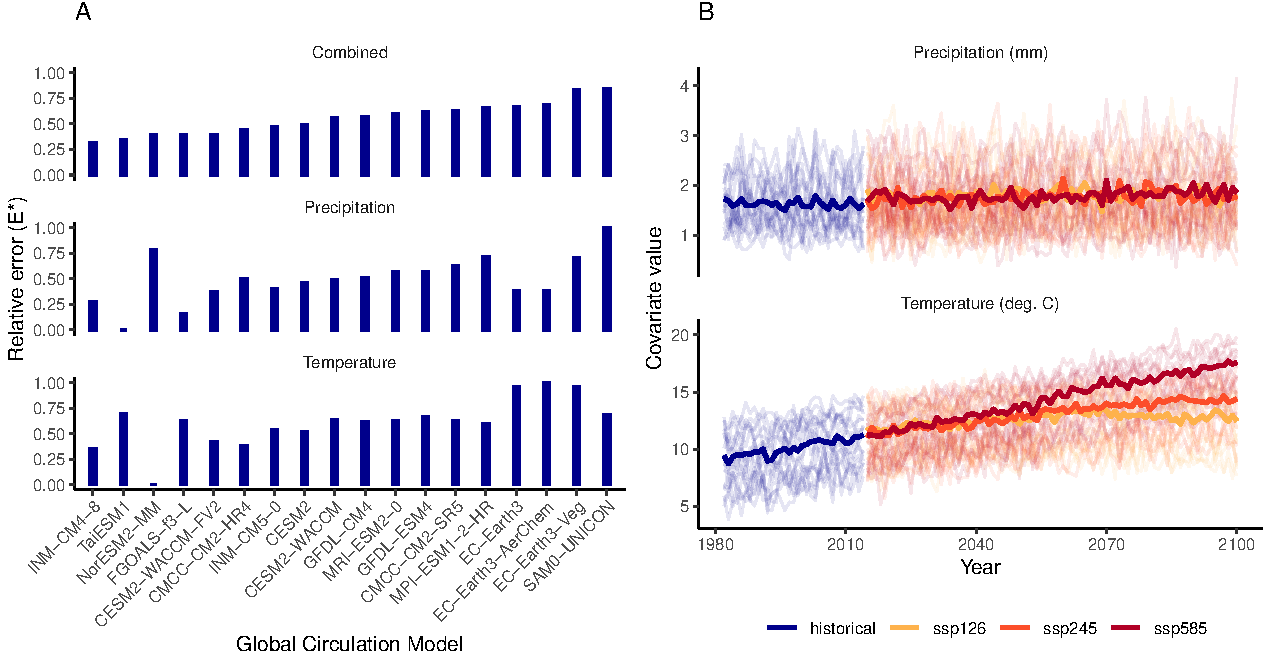
\includegraphics{sageCastManuscript_files/figure-latex/gcm-ranks-1.pdf}
\caption{\label{fig:gcm-ranks}(A) Relative errors of global circulation models (GCMs) when comparing historical projections to observed PRISM climate data within sage-grouse core areas in Wyoming, USA for the period 1985-2018. Values in the top panel (Combined) were subtracted from 1 and normalized for use as model weights when projecting sagebrush dynamics. GCMs are ordered from lowest (left) to highest (right) combined error. (B) Climate change projections for Greater South Pass (north) from all GCMs (light lines) and the weighted average of climate projections, which are proportional to the relative errors in panel A. Shared socio-economic pathways (SSPs): ssp126 (low future carbon emissions), ssp245 (intermediate future carbon emissions), and ssp585 (high future carbon emissions).}
\end{figure}

\hypertarget{statistical-model-evaluation}{%
\subsection{Statistical model evaluation}\label{statistical-model-evaluation}}

Convergence diagnostics indicated that most MCMC chains converged on their stationary distributions (upper 0.95 quantiles of \(\hat{R}\) \textless{} 1.1 for all parameters; Appendix S1: Tables S1 - S39).
This was true except for the model for Elk Basin West (Appendix S1: Table S9).
Results from Elk Basin West are not further discussed because the MCMC chains did not converge and because the model failed the posterior predictive checks described next.
Most Bayesian \emph{P}-values indicated no lack-of-fit because they were greater than 0.05 and less than 0.95 for both the spatial (\(P_B^{\text{space}}\)) and temporal (\(P_B^{\text{time}}\)) test statistic \emph{P}-values (Appendix S1: Table S40).
The \(P_B^{\text{time}}\) value for Elk Basin West indicated lack-of-fit.
The \(P_B^{\text{space}}\) values for Powder, Sage, Seedskadee, and Uinta indicated lack-of-fit.
We do not present any further results on these sites because inference from their models cannot be trusted (Hobbs and Hooten 2015).

\hypertarget{parameter-estimates}{%
\subsection{Parameter estimates}\label{parameter-estimates}}

Posterior distributions for all model parameters for each core area are presented in the online supporting information (Appendix S1: Figs. S1 - S39; Appendix S1: Tables S41 - S79).
The posterior distributions of equilibrium cover \(\left(y' = e^{\beta_1 / \left(1 - \beta_2 \right)}\right)\) for each core area contain the observed mean cover values, except for a few core areas (Appendix S1: Fig. S40).
Cases where mean observed cover does not fall within estimated equilibrium cover suggest that climate effects over the past 30 years or other disturbances not modeled (but potentially reflected in random year effects) have kept cover from reaching the equilibrium.
Climate effects are described as sensitivities below.
Results from the colonization probability model used for future simulations are presented in the online supporting information (Appendix S1: Table S80).

\hypertarget{sensitivities}{%
\subsection{Sensitivities}\label{sensitivities}}

All core areas showed some sensitivity to climate drivers (Fig. \ref{fig:sensitivities}).
The majority of core areas had a positive sensitivity to temperature and negative sensitivity to precipitation (n = 16; Fig. \ref{fig:sen-scatter}).
The most consistent pattern was a positive effect of temperature on sagebrush performance (n = 24 out of 34 total {[}70\%{]}; Figs. \ref{fig:sensitivities}, \ref{fig:sen-scatter}).

\begin{figure}
\centering
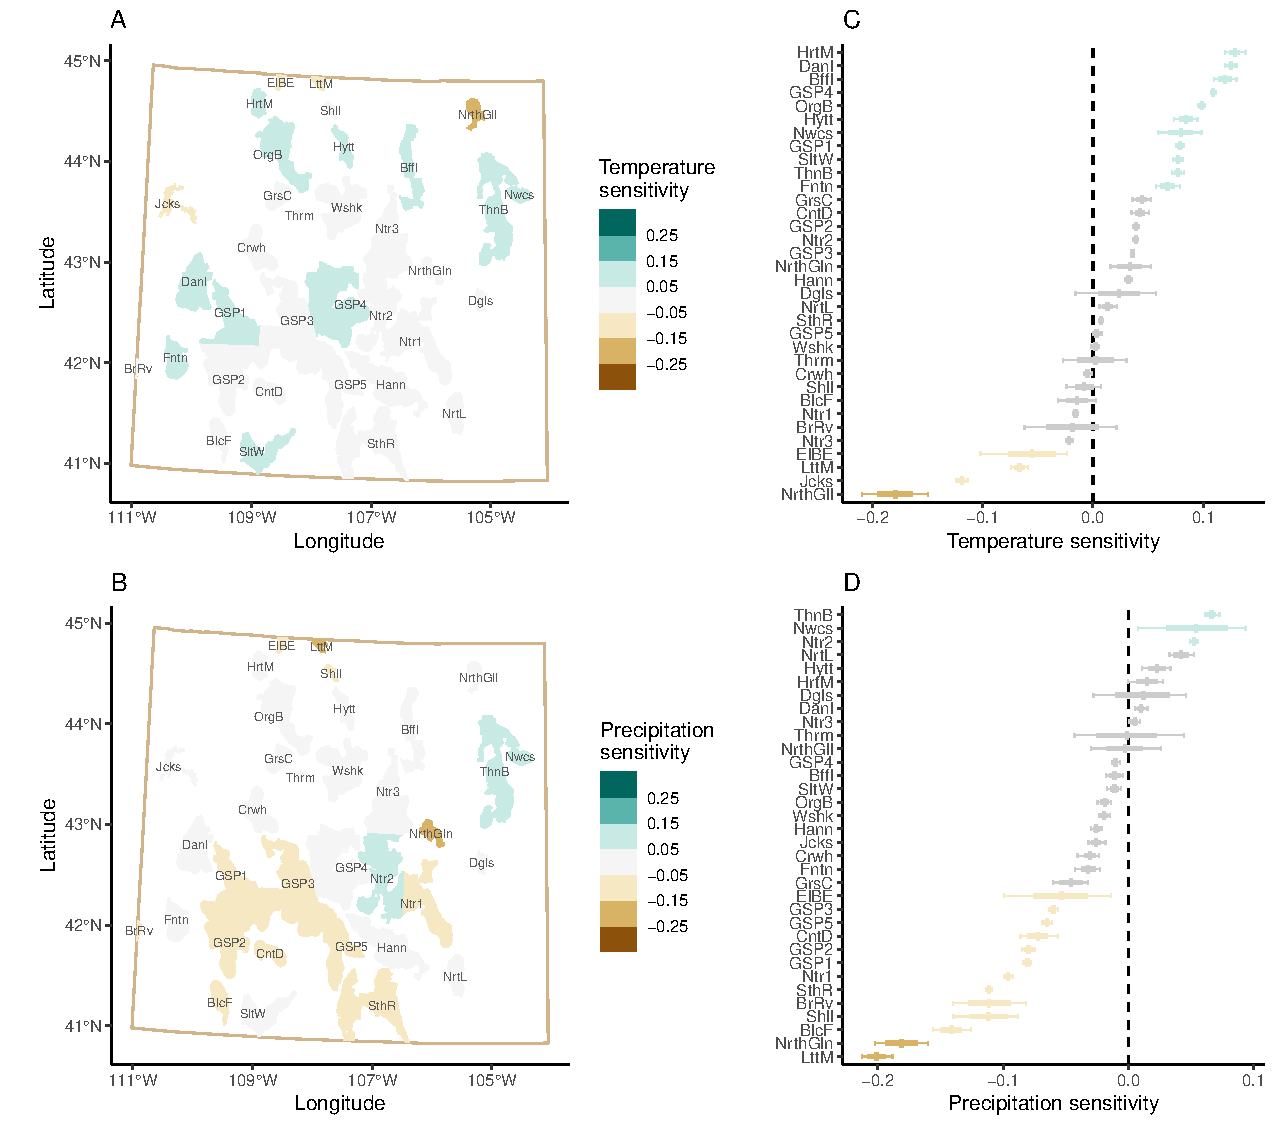
\includegraphics{sageCastManuscript_files/figure-latex/sensitivities-1.pdf}
\caption{\label{fig:sensitivities}Sensitivity of sagebrush cover to average spring-through-summer temperature and average spring-through-summer precipitation. Maps show the mean of the posterior distribution of sensitivity to temperature (A) and precipitation (B) for each sage-grouse core area in Wyoming, USA. Dark grey core areas are those whose models did not pass posterior predictive checks. Panels to the right of the maps show the mean (crosshairs), 95\% Bayesian credible interval (bold lines), and range of the posterior distributions (whiskers) of sensitivity to temperature (C) and precipitation (D) for each core area. Colors indicate positive (greens), negative (browns), and negligble (light grey) sensitivity. Sensitivity is defined as the log change in cover relative to equilibrium cover when a +1 standard deviation perturbation is applied to the climate effect in the fitted model for each core area.}
\end{figure}

\begin{figure}
\centering
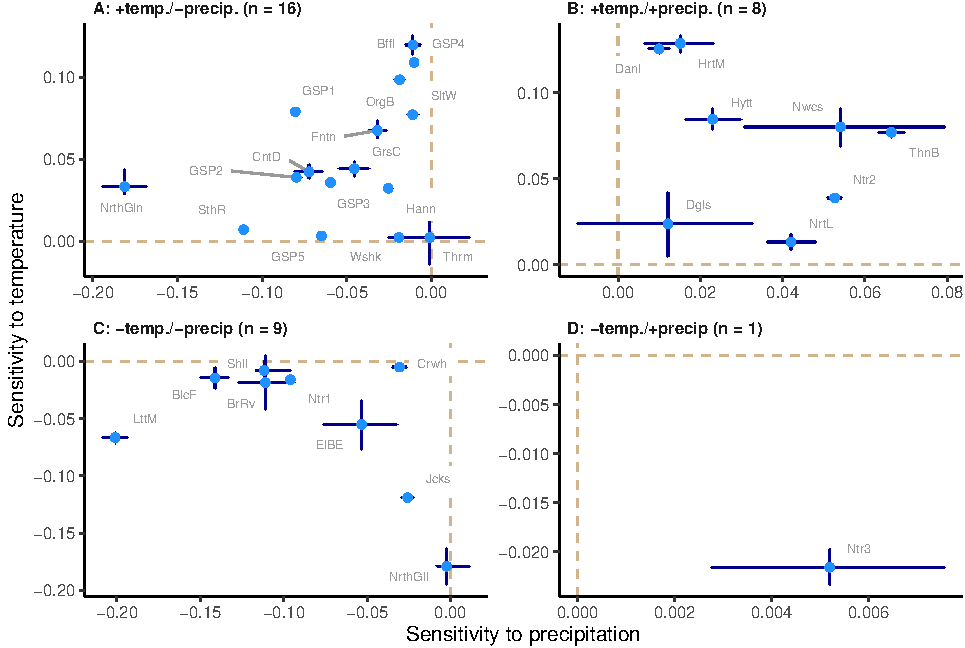
\includegraphics{sageCastManuscript_files/figure-latex/sen-scatter-1.pdf}
\caption{\label{fig:sen-scatter}Sensitivity of each sage-grouse core area in Wyoming, USA to temperature and precipitation grouped by positive and negative responses to each climate driver. (A) Core areas with negative sensitivity to precipitation and positive sensitivity to temperature. (B) Core areas with positive sensitivity to precipitation and temperature, (C) Core areas with a negative sensitivity to precipitation and temperature. (D) Core areas with a positive sensitivity to precipitation and a negative sensitivity to temperature. Points show the posterior means and whiskers show the 95\% Bayesian credible intervals. Dashed tan lines show where sensitivity equals zero. The panel labels also indicate the number of core areas (n) in each sensitivity quadrant.}
\end{figure}

Averaging over all the posterior distributions for the precipitation and temperature sensitivities, we found that overall average sensitivity to precipitation was negative: mean = -0.036 (pseudo 95\% Bayesian credible interval (BCI) = -0.038, -0.034).
The overall average sensitivity to temperature was positive: mean = 0.025 (pseudo 95\% BCI = 0.023, 0.027).
Note that we refer to the confidence intervals as ``pseudo BCIs'' because the average of the posteriors is not strictly the cross-core area posterior distribution.
Nonetheless, the average values do inform the general pattern.
The variance of the overall average sensitivities should be viewed as the variance of the mean sensitivity, not as the variance of sensitivity magnitudes across core areas.

\hypertarget{projections}{%
\subsection{Projections}\label{projections}}

Projections of sagebrush cover into the future are primarily driven by the sensitivity of cover to temperature and the magnitude of temperature change.
This is because precipitation is not projected to increase or decrease much in the future in Wyoming (Fig. \ref{fig:gcm-ranks}B).
Because most core areas had a positive sensitivity to temperature, sagebrush cover is projected to increase at most core areas (Fig. \ref{fig:projections}).
Projections of sagebrush cover are similar across GCM scenarios until about mid-century, at which point ssp585 projections diverge if temperature has a large (positive or negative) effect on interannual changes in sagebrush cover (Fig. \ref{fig:projections}).

More core areas were projected to increase in sagebrush cover (n = 21 for ssp126; n = 22 for ssp245 and ssp585) than decrease (n = 13 for ssp126; n = 12 for ssp245 and ssp585) and the magnitude of increases was greater than decreases for each GCM scenario.
For decreases, the median percent difference between average cover in 2018 and average cover in 2100 was -9\% for ssp126, -18\% for ssp245, and -24\% for ssp585.
For increases, the median percent difference between average cover in 2018 and average cover in 2100 was 17\% for ssp126, 34\% for ssp245, and 79\% for ssp585.
The percent differences show that projected increases in sagebrush cover are nearly twice the magnitude of projected decreases for each GCM scenario, on average.
Summing across core areas, 41711 - 45474 \(\text{km}^2\) of land is projected to experience increases in sagebrush cover on average, depending on GCM scenario.
In contrast, 12978 - 16740 \(\text{km}^2\) of land is projected to experience decreases in sagebrush cover on average, depending on GCM scenario.

Figure \ref{fig:spatial-projections} shows projections over time and space for the Salt Wells core area (as an example) under the ssp585 climate forcing scenario.
Salt Wells is located in southwestern Wyoming (Fig. \ref{fig:sensitivities}).
Spatial heterogeneity is maintained because of the spatial offset included in the model, but heterogeneity is smoothed somewhat, resulting in slightly lower spatial variance.
Lower spatial variance can impact the calculation of the proportion of grid cells with cover over or under the nesting and summer habitat targets.
At this core area, projections show sagebrush increasing slightly over most of the area, but with large increases in cover in the western edge of the core area. (Fig. \ref{fig:spatial-projections}).

Notable declines in sagebrush cover are projected for Bear River (BrRv), Elk Basin East (ElBE), Jackson (Jcks), Little Mountain (LttM), and North Gillette (NrthGll) core areas (Fig. \ref{fig:projections}).
These same core areas may become suboptimal for sage-grouse over the long-term, as projections suggest the proportion of cells in Bear River, Little Mountain, and Jackson that exceed the sage-grouse nesting target (Appendix S1: Table S81) drop below 50\% at some point in the future (Figs. \ref{fig:nesting-targs} and \ref{fig:lambda-compares}B).
Twelve core areas are projected to switch from supoptimal to optimal for sage-grouse by crossing the 50\% threshold in the future (Figs. \ref{fig:nesting-targs} and \ref{fig:lambda-compares}D).
Results based on summer habitat cover targets are similar (Appendix S1: Fig. S41).
The most common projection (n = 16) is for currently suboptimal core areas to remain suboptimal, even though most will experience gains in sagebrush cover (Fig. \ref{fig:lambda-compares}).

Most sage-grouse population growth rates have confidence intervals that overlap one, indicating a stable population (Fig. \ref{fig:lambda-compares}).
However, the mean growth rates suggest that 12 of the 16 core areas projected to remain suboptimal already have declining sage-grouse populations (Fig. \ref{fig:lambda-compares}C).
Ten of the 12 core areas projected to switch from suboptimal to optimal have mean sage-grouse population growth rates that are negative (Fig. \ref{fig:lambda-compares}D).

\begin{figure}
\centering
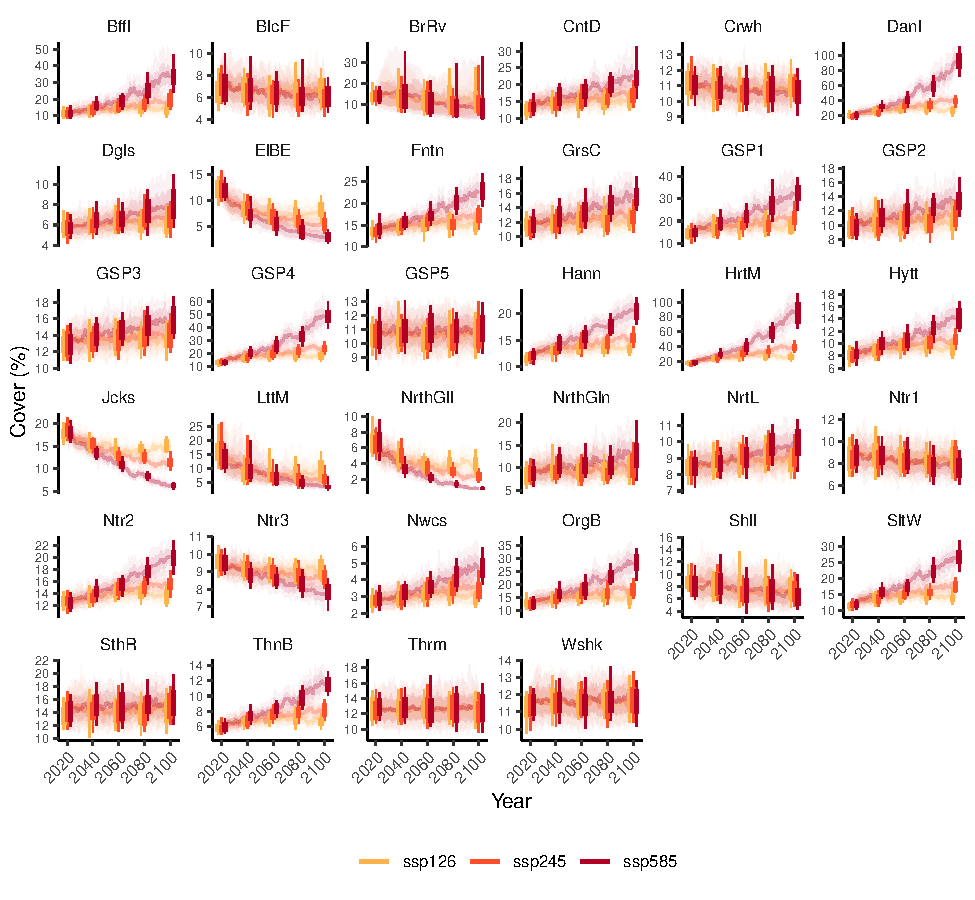
\includegraphics{sageCastManuscript_files/figure-latex/projections-1.pdf}
\caption{\label{fig:projections}Projections of sagebrush percent cover from 2018 to 2100 under three climate change scenarios (ssp indicated by colors) for each sage-grouse core area in Wyoming, USA. The solid line is the median of the posterior predictive distribution; light shaded ribbon bounds the 68\% Bayesian credible interval (BCI); very light shaded ribbon bounds the 95\% BCI. Box and whiskers show the 68\% (boxes) and 95\% (whiskers) BCIs at discrete time horizons of 2020, 2040, 2060, 2080, and 2100. The y-axis scale differs across plots. Shared socio-economic pathways (SSPs): ssp126 (low future carbon emissions), ssp245 (intermediate future carbon emissions), and ssp585 (high future carbon emissions).}
\end{figure}

\begin{figure}
\centering
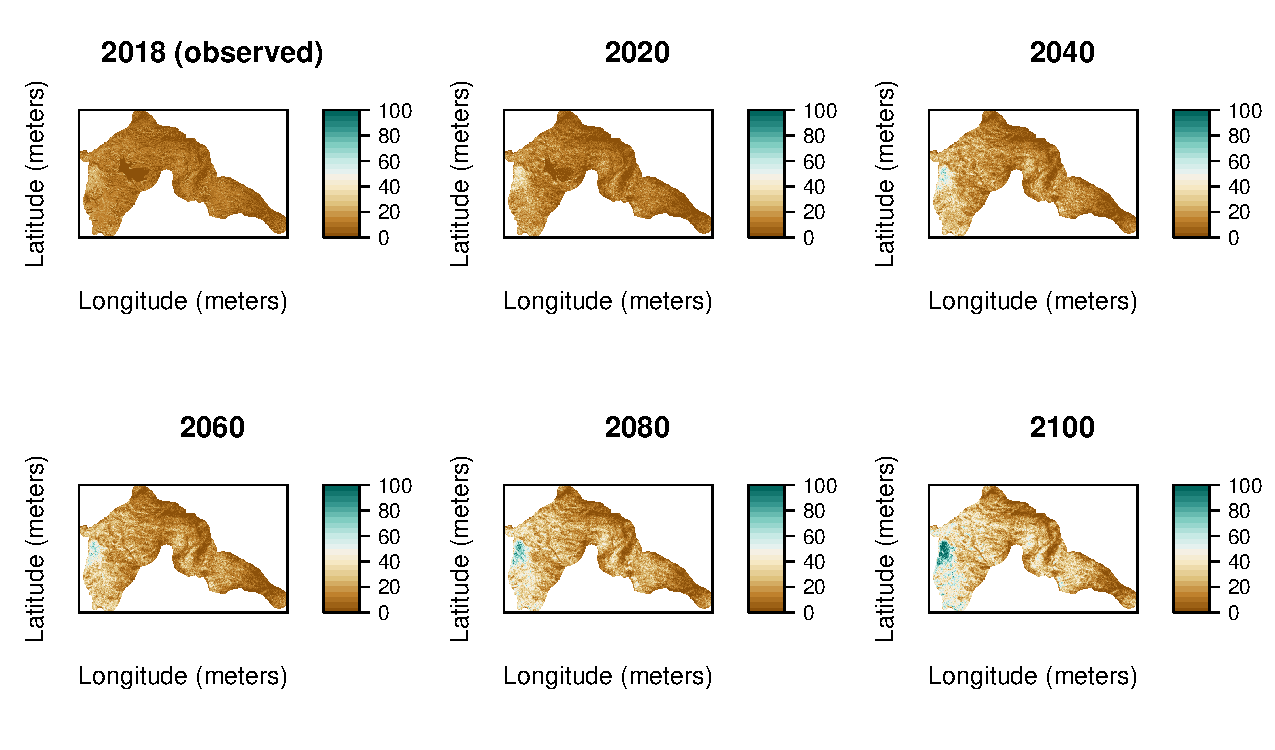
\includegraphics{sageCastManuscript_files/figure-latex/spatial-projections-1.pdf}
\caption{\label{fig:spatial-projections}Projections of sagebrush percent cover (color bars indicate percent cover value) over space and time for the Salt Wells (SltW) sage-grouse core area in southwestern Wyoming, USA. Projections are plotted from a single ensemble member (one parameter set) and using the ssp585 (high future carbon emissions) climate forcing scenario.}
\end{figure}

\begin{figure}
\centering
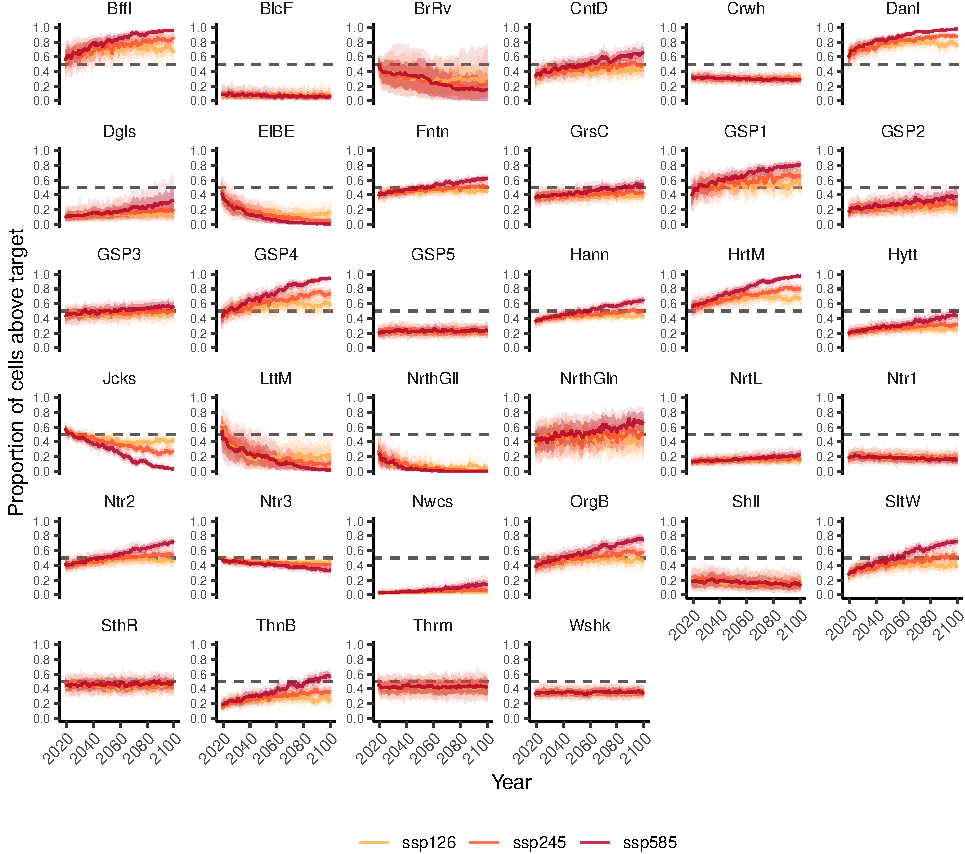
\includegraphics{sageCastManuscript_files/figure-latex/nesting-targs-1.pdf}
\caption{\label{fig:nesting-targs}Projections of the proportion of 100-meter cells within a core area where sagebrush percent cover exceeds the sage-grouse nesting threshold defined for each sage-grouse core area in Wyoming, USA. The solid line is the median of the posterior predictive distribution; light shaded ribbon bounds the 68\% Bayesian credible interval (BCI); very light shaded ribbon bounds the 95\% BCI. The dashed horizontal line shows where the proportion of cells is equal to 50\% of the area. Shared socio-economic pathways (SSPs): ssp126 (low future carbon emissions), ssp245 (intermediate future carbon emissions), and ssp585 (high future carbon emissions).}
\end{figure}

\begin{figure}
\centering
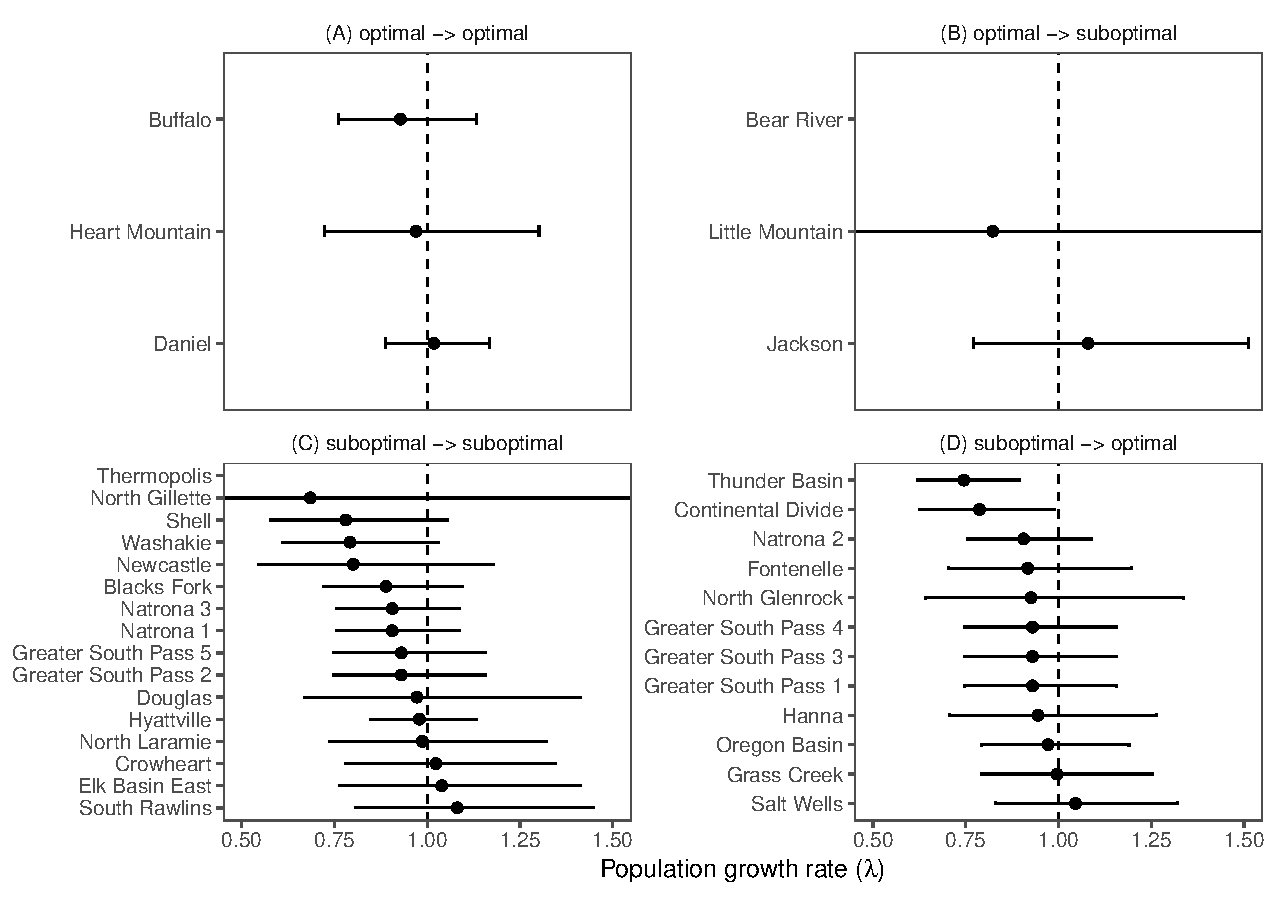
\includegraphics{sageCastManuscript_files/figure-latex/lambda-compares-1.pdf}
\caption{\label{fig:lambda-compares}Sage-grouse population growth rates from Edmunds et al.~(2018; Erratum 2018) for each sage-grouse core area in Wyoming, USA (point = estimate, whiskers = 95\% confidence interval {[}CI{]}), grouped by whether (A) the core area is currently more suitable and projected to remain more suitable, (B) currently more suitable and projected to become less suitable, (C) currently less suitable and projected to remain less suitable, and (D) currently less suitable and projected to become more suitable. `More suitable' is defined as over 50\% of cells with cover over the nesting threshold. `Less suitable' is defined as fewer than 50\% of cells with cover over the nesting threshold.}
\end{figure}

\hypertarget{discussion}{%
\section{Discussion}\label{discussion}}

Projections of sagebrush cover represent the combined effect of sensitivity to the climate drivers and the magnitude of change expected in the climate driver in the future.
We found that sagebrush performance at most core areas showed positive sensitivity to temperature and negative sensitivity to precipitation.
Because average temperature is expected to increase in Wyoming in the future and average precipitation is expected to remain relatively constant, we project an increase in sagebrush cover at most core areas across Wyoming.
Moreover, projected increases were larger in magnitude than decreases and increases were projected on about four times larger land area (about 45,000 \(\text{km}^2\) expected to experience increases relative to about 13,000 \(\text{km}^2\) expected to experience decreases, on average).
This finding suggests that few core areas are ``lost causes'' in terms of maintaining existing sagebrush cover in the future.
Continued conservation of these core areas has the potential to increase the extent of the landscape with sagebrush cover exceeding the nesting and summer habitat thresholds (Figs. \ref{fig:nesting-targs} and S41).
Even when the threshold is not projected to be exceeded, sagebrush cover is most commonly projected to increase.

The most common climate response across the core areas was a positive effect of temperature on sagebrush performance.
This finding is consistent with theoretical and empirical research suggesting that plants at the cold-limited edge of their distribution may benefit from global climate change (Amburgey et al. 2018, Kleinhesselink and Adler 2018, Renwick et al. 2018b).
The finding is also consistent with results across a broader range of the sagebrush distribution using the BIT data but with more and different climate predictors (Rigge et al. 2021).
Recent mechanistic modeling across the sagebrush biome also suggests that increases in temperature will benefit sagebrush in high elevation portions of its range, like Wyoming (Palmquist et al. 2021).
Palmquist et al. (2021) showed that soil moisture will likely remain adequate under a warming climate in cold, winter-wet areas where sagebrush performance is temperature-limited.
Other studies have also found positive effects of temperature increases at high elevation sagebrush sites, likely due to earlier snowmelt and a longer growing season (Perfors et al. 2003, Harte et al. 2015).
Our statistical models appear to reflect these underlying mechanistic explanations at a majority of core areas.
A negative sensitivity to above average spring-through-summer precipitation combined with a positive sensitivity to spring-through-summer temperature could reflect sagebrush responding negatively to late season snow in colder years and positively to earlier snow melt in warmer years.
The negative sensitivity of sagebrush to precipitation is confusing, but the negative sensitivity could be reflecting an interaction we failed to model.
Last, variable responses to above- and below-average precipitation is expected across large regions with variable soil depths (Germino and Reinhardt 2014).

Climate responses were not uniform across core areas, however.
The models showed positive and negative responses to both precipitation and temperature annual anomolies.
Opposing effects of weather on sagebrush performance are not uncommon (Renwick et al. 2018b, Palmquist et al. 2021).
Regional, landscape, and local gradients in average climate (Kleinhesselink and Adler 2018), soil conditions (Schlaepfer et al. 2012, Germino and Reinhardt 2014), and subspecies composition (Rosentreter 2005) can have a strong influence on sagebrush responses to weather and climate.

The biggest limiation of our study is that we only quantified the direct effects of climate on sagebrush performance.
Indirect effects of climate change and other non-climate related effects might be more influential.
In particular, the fire-cheatgrass invasion cycle has been implicated as the major driver of sagebrush loss across most of its historical range.
Recent modeling suggests that parts of Wyoming may become more suitable for cheatgrass but that cheatgrass invasion could be limited if disturbances that reduce native grass and shrub cover are limited (Palmquist et al. 2021).
Hotter and drier conditions in the future will likely increase fire risk throughout Wyoming shrublands, meaning it could be difficult to limit cheatgrass invasion if fires become widespread.
Schlaepfer et al. (2021) found a similar result in terms of sagebrush regeneration: regeneration will likely remain possible under a warming climate alone, but the fire-cheatgrass interaction will likely limit sagebrush persistence.
Nonetheless, our results corroborate those of Palmquist et al. (2021) and Schlaepfer et al. (2021) by suggesting that climate change alone should benefit, or at least not significantly disadvantage, sagebrush in Wyoming.

A second limitation is that we implicitly assume that the relationships between sagebrush percent cover and temperature and precipitation are log-linear.
That is, by using the statistical models to project cover into the future, we are assuming that the relationships quantified from historical data will be maintained in the future.
It is certainly possible that sagebrush performance will plateau at temperatures and precipitation levels outside of the historical range of variability, either because of physiological limits or evolutionary adaptation (Adler et al. 2020).
Evolutionary adaptation represents just one of many possible ``slow'' processes that impact our ability to make projections using short-term data that likely represent ``fast'' processes (Adler et al. 2020).
Sagebrush are slow to recover from extreme events like drought that cause die-offs, representing another slow process potentially not captured by our models.
Therefore, our models likely miss the impact of such extreme events.

Our sagebrush projections can be used as part of a decision-support toolbox for managers in Wyoming.
The projections are also useful for generating hypotheses and scientific questions.
For example, what conditions lead to two core areas in the same region having divergent responses to temperature (North Gillette versus Thunder Basin, Fig. \ref{fig:sensitivities}A)?
Observational and experimental studies could help explain the divergent responses.
So too could targeted modeling studies that use more climate and environmental covariates then we used here.
Such explanations are critical to guide region-wide management of sagebrush landscapes in the face of climate change and potential cheatgrass invasion.

\hypertarget{implications-for-sage-grouse-management}{%
\section{Implications for sage-grouse management}\label{implications-for-sage-grouse-management}}

Sage-grouse are sagebrush-obligate species, meaning any increase in sagebrush cover likely benefits sage-grouse.
However, other factors not considered here can affect habitat quality, including herbaceous vegetation, structure, and configuration of sagebrush on the landscape, and disturbances Fedy et al. (2014){]}, in addition to higher temperatures (Blomberg et al. 2012, Lundblad et al. 2022).
We also acknowledge that our use of thresholds to determine whether habitat was ``optimal'\,' for sage-grouse, while consistent with the Sage-grouse Habitat Assessment Framework (Stiver et al. 2015), may not correspond with more local trends in demography (Smith et al. 2020).
Indeed, most core areas we classified as currently ``suboptimal'' had stable population trends (Edmunds et al. 2018), whereas fewer core areas currently had ``optimal'' levels of sagebrush cover (Fig. \ref{fig:lambda-compares}).
Therefore, we emphasize that while the thresholds used here were useful for a relative comparison of habitat status across core areas, studying effects of sagebrush cover on demographics such as population trends, at relevant spatial scales (Monroe et al. 2022), would provide a more direct assessment of habitat quality for sage-grouse (and implications of climate change).

Nevertheless, not all core areas are projected to increase in sagebrush cover.
But the magnitude of increase and the area over which we project increases far outweigh projected declines.
These results highlight the importance of active and adaptive management in Wyoming's sage-grouse core areas, which contain about 37\% of all sage-grouse (Fedy et al. 2014).
Our results suggest that climate change per se is not going to cause declines in sagebrush in Wyoming.
Therefore, management actions aimed at reducing cheatgrass invasion and limiting disturbances in core areas might help mitigate the negative, indirect impacts of climate change.
In part, this is good news because managing disturbances and plant invasions is more feasible than managing global climate change.

Even still, effectively conserving all of the core areas may not be enough to ensure sage-grouse conservation (Hannah et al. 2007, Monzón et al. 2011).
Sage-grouse use vast areas outside of the core areas as well, particularly in the apex of the population cycles (Heinrichs et al. 2019).
Sage-grouse require diverse resource compositions across life stages, with an upper limit of annual life-time home ranges estimated at \textasciitilde2975 km\(^2\) (Connelly et al. 2000b, Connelly et al. 2000a).
This suggests that maintaining large intact landscapes inside and outside of core areas (Heinrichs et al.~2019) can help ensure viable sage-grouse populations persist.
Our models help to identify sagebrush habitats that are likely to persist into the future given climate change, highlighting areas for potential long-term preservation and protection.
Areas with projected sagebrush declines may need to be more closely managed.

\hypertarget{acknowledgements}{%
\section{Acknowledgements}\label{acknowledgements}}

This study was funded by the Bureau of Land Management and the U.S. Geological Survey.
Any use of trade, firm, or product names is for descriptive purposes only and does not imply endorsement by the U.S. government.
We thank Robert Shriver and Darren Long for reviewing preliminary versions of the manuscript.

\hypertarget{references}{%
\section{References}\label{references}}

\setlength{\parindent}{-0.2in}
\setlength{\leftskip}{0.2in}
\setlength{\parskip}{8pt}

\noindent

\hypertarget{refs}{}
\begin{CSLReferences}{1}{0}
\leavevmode\vadjust pre{\hypertarget{ref-adler_matching_2020}{}}%
Adler, P. B., E. P. White, and M. H. Cortez. 2020. \href{https://doi.org/10.1111/ecog.05271}{Matching the forecast horizon with the relevant spatial and temporal processes and data sources}. Ecography 43:1729--1739.

\leavevmode\vadjust pre{\hypertarget{ref-amburgey_range_2018}{}}%
Amburgey, S. M., D. A. W. Miller, E. H. C. Grant, T. A. G. Rittenhouse, M. F. Benard, J. L. Richardson, M. C. Urban, W. Hughson, A. B. Brand, C. J. Davis, C. R. Hardin, P. W. C. Paton, C. J. Raithel, R. A. Relyea, A. F. Scott, D. K. Skelly, D. E. Skidds, C. K. Smith, and E. E. Werner. 2018. \href{https://doi.org/10.1111/gcb.13817}{Range position and climate sensitivity: {The} structure of among-population demographic responses to climatic variation}. Global Change Biology 24:439--454.

\leavevmode\vadjust pre{\hypertarget{ref-balch_introduced_2013}{}}%
Balch, J. K., B. A. Bradley, C. M. D'Antonio, and J. Gómez-Dans. 2013. \href{https://doi.org/10.1111/gcb.12046}{Introduced annual grass increases regional fire activity across the arid western {USA} (1980--2009)}. Global Change Biology 19:173--183.

\leavevmode\vadjust pre{\hypertarget{ref-blomberg_characteristics_2012}{}}%
Blomberg, E. J., J. S. Sedinger, M. T. Atamian, and D. V. Nonne. 2012. \href{https://doi.org/10.1890/ES11-00304.1}{Characteristics of climate and landscape disturbance influence the dynamics of greater sage-grouse populations}. Ecosphere 3:art55.

\leavevmode\vadjust pre{\hypertarget{ref-boettiger_optimal_2016}{}}%
Boettiger, C., M. Bode, J. N. Sanchirico, J. LaRiviere, A. Hastings, and P. R. Armsworth. 2016. \href{https://doi.org/10.1890/15-0236}{Optimal management of a stochastically varying population when policy adjustment is costly}. Ecological Applications 26:808--817.

\leavevmode\vadjust pre{\hypertarget{ref-bradley_regional_2009}{}}%
Bradley, B. A. 2009. \href{https://doi.org/10.1111/j.1365-2486.2008.01709.x}{Regional analysis of the impacts of climate change on cheatgrass invasion shows potential risk and opportunity}. Global Change Biology 15:196--208.

\leavevmode\vadjust pre{\hypertarget{ref-cardinale_biodiversity_2012}{}}%
Cardinale, B. J., J. E. Duffy, A. Gonzalez, D. U. Hooper, C. Perrings, P. Venail, A. Narwani, G. M. Mace, D. Tilman, D. A. Wardle, A. P. Kinzig, G. C. Daily, M. Loreau, J. B. Grace, A. Larigauderie, D. S. Srivastava, and S. Naeem. 2012. \href{https://doi.org/10.1038/nature11148}{Biodiversity loss and its impact on humanity}. Nature 486:59--67.

\leavevmode\vadjust pre{\hypertarget{ref-chambers_what_2007}{}}%
Chambers, J. C., B. A. Roundy, R. R. Blank, S. E. Meyer, and A. Whittaker. 2007. \href{https://doi.org/10.1890/05-1991}{What {Makes} {Great} {Basin} {Sagebrush} {Ecosystems} {Invasible} by {Bromus} {Tectorum}?} Ecological Monographs 77:117--145.

\leavevmode\vadjust pre{\hypertarget{ref-clark_ecological_2001}{}}%
Clark, J. S., S. R. Carpenter, M. Barber, S. Collins, A. Dobson, J. A. Foley, D. M. Lodge, M. Pascual, R. Pielke, W. Pizer, C. Pringle, W. V. Reid, K. A. Rose, O. Sala, W. H. Schlesinger, D. H. Wall, and D. Wear. 2001. \href{https://doi.org/10.1126/science.293.5530.657}{Ecological {Forecasts}: {An} {Emerging} {Imperative}}. Science 293:657--660.

\leavevmode\vadjust pre{\hypertarget{ref-conn_using_2015}{}}%
Conn, P. B., D. S. Johnson, J. M. V. Hoef, M. B. Hooten, J. M. London, and P. L. Boveng. 2015. \href{https://doi.org/10.1890/14-0959.1}{Using spatiotemporal statistical models to estimate animal abundance and infer ecological dynamics from survey counts}. Ecological Monographs 85:235--252.

\leavevmode\vadjust pre{\hypertarget{ref-conn_guide_2018}{}}%
Conn, P. B., D. S. Johnson, P. J. Williams, S. R. Melin, and M. B. Hooten. 2018. \href{https://doi.org/10.1002/ecm.1314}{A guide to {Bayesian} model checking for ecologists}. Ecological Monographs 88:526--542.

\leavevmode\vadjust pre{\hypertarget{ref-connelly_conservation_2000}{}}%
Connelly, J. W., S. T. Knick, M. A. Schroeder, and S. J. Stiver. 2000a. Conservation assessment of greater sage-grouse and sagebrush habitats. Western Association of Fish; Wildlife Agencies, Cheyenne, Wyoming.

\leavevmode\vadjust pre{\hypertarget{ref-connelly_response_2000}{}}%
Connelly, J. W., K. P. Reese, R. A. Fischer, and W. L. Wakkinen. 2000b. \href{https://www.jstor.org/stable/4617288}{Response of a {Sage} {Grouse} {Breeding} {Population} to {Fire} in {Southeastern} {Idaho}}. Wildlife Society Bulletin (1973-2006) 28:90--96.

\leavevmode\vadjust pre{\hypertarget{ref-davies_saving_2011}{}}%
Davies, K. W., C. S. Boyd, J. L. Beck, J. D. Bates, T. J. Svejcar, and M. A. Gregg. 2011. \href{https://doi.org/10.1016/j.biocon.2011.07.016}{Saving the sagebrush sea: {An} ecosystem conservation plan for big sagebrush plant communities}. Biological Conservation 144:2573--2584.

\leavevmode\vadjust pre{\hypertarget{ref-dietze_iterative_2018}{}}%
Dietze, M. C., A. Fox, L. M. Beck-Johnson, J. L. Betancourt, M. B. Hooten, C. S. Jarnevich, T. H. Keitt, M. A. Kenney, C. M. Laney, L. G. Larsen, H. W. Loescher, C. K. Lunch, B. C. Pijanowski, J. T. Randerson, E. K. Read, A. T. Tredennick, R. Vargas, K. C. Weathers, and E. P. White. 2018. \href{https://doi.org/10.1073/pnas.1710231115}{Iterative near-term ecological forecasting: {Needs}, opportunities, and challenges}. Proceedings of the National Academy of Sciences 115:1424--1432.

\leavevmode\vadjust pre{\hypertarget{ref-edmunds_greater_2018}{}}%
Edmunds, D. R., C. L. Aldridge, M. S. O'Donnell, and A. P. Monroe. 2018. \href{https://doi.org/10.1002/jwmg.21386}{Greater sage-grouse population trends across {Wyoming}}. The Journal of Wildlife Management 82:397--412.

\leavevmode\vadjust pre{\hypertarget{ref-noauthor_erratum_2018}{}}%
\href{https://doi.org/10.1002/jwmg.21560}{Erratum}. 2018. The Journal of Wildlife Management 82:1808--1808.

\leavevmode\vadjust pre{\hypertarget{ref-eyring_overview_2016}{}}%
Eyring, V., S. Bony, G. A. Meehl, C. A. Senior, B. Stevens, R. J. Stouffer, and K. E. Taylor. 2016. \href{https://doi.org/10.5194/gmd-9-1937-2016}{Overview of the {Coupled} {Model} {Intercomparison} {Project} {Phase} 6 ({CMIP6}) experimental design and organization}. Geoscientific Model Development 9:1937--1958.

\leavevmode\vadjust pre{\hypertarget{ref-farber_linking_2006}{}}%
Farber, S., R. Costanza, D. L. Childers, J. Erickson, K. Gross, M. Grove, C. S. Hopkinson, J. Kahn, S. Pincetl, A. Troy, P. Warren, and M. Wilson. 2006. \href{https://doi.org/10.1641/0006-3568(2006)056\%5B0121:LEAEFE\%5D2.0.CO;2}{Linking {Ecology} and {Economics} for {Ecosystem} {Management}}. BioScience 56:121--133.

\leavevmode\vadjust pre{\hypertarget{ref-fedy_habitat_2014}{}}%
Fedy, B. C., K. E. Doherty, C. L. Aldridge, M. O'Donnell, J. L. Beck, B. Bedrosian, D. Gummer, M. J. Holloran, G. D. Johnson, N. W. Kaczor, C. P. Kirol, C. A. Mandich, D. Marshall, G. Mckee, C. Olson, A. C. Pratt, C. C. Swanson, and B. L. Walker. 2014. \href{https://doi.org/10.1002/wmon.1014}{Habitat prioritization across large landscapes, multiple seasons, and novel areas: {An} example using greater sage-grouse in {Wyoming}}. Wildlife Monographs 190:1--39.

\leavevmode\vadjust pre{\hypertarget{ref-gelman_data_2006}{}}%
Gelman, A., and J. Hill. 2006. Data {Analysis} {Using} {Regression} and {Multilevel}/{Hierarchical} {Models}. Cambridge University Press.

\leavevmode\vadjust pre{\hypertarget{ref-gelman_inference_1992}{}}%
Gelman, A., and D. B. Rubin. 1992. \href{https://doi.org/10.1214/ss/1177011136}{Inference from {Iterative} {Simulation} {Using} {Multiple} {Sequences}}. Statistical Science 7:457--472.

\leavevmode\vadjust pre{\hypertarget{ref-germino_desert_2014}{}}%
Germino, M. J., and K. Reinhardt. 2014. \href{https://doi.org/10.1111/1365-2745.12266}{Desert shrub responses to experimental modification of precipitation seasonality and soil depth: Relationship to the two-layer hypothesis and ecohydrological niche}. Journal of Ecology 102:989--997.

\leavevmode\vadjust pre{\hypertarget{ref-guo_rstan_2020}{}}%
Guo, J., J. Gabry, B. Goodrich, S. Weber, D. Lee, K. Sakrejda, M. Martin, T. of C. University, O. Sklyar (R/cxxfunplus.R), T. R. C. Team (R/pairs.R, R/dynGet.R), J. Oehlschlaegel-Akiyoshi (R/pairs.R), J. Maddock (gamma.hpp), P. Bristow (gamma.hpp), N. Agrawal (gamma.hpp), C. Kormanyos (gamma.hpp), and B. Steve. 2020, July. \href{https://CRAN.R-project.org/package=rstan}{Rstan: {R} {Interface} to {Stan}}.

\leavevmode\vadjust pre{\hypertarget{ref-hannah_protected_2007}{}}%
Hannah, L., G. Midgley, S. Andelman, M. Araújo, G. Hughes, E. Martinez-Meyer, R. Pearson, and P. Williams. 2007. \href{https://doi.org/10.1890/1540-9295(2007)5\%5B131:PANIAC\%5D2.0.CO;2}{Protected area needs in a changing climate}. Frontiers in Ecology and the Environment 5:131--138.

\leavevmode\vadjust pre{\hypertarget{ref-harte_convergent_2015}{}}%
Harte, J., S. R. Saleska, and C. Levy. 2015. \href{https://doi.org/10.1111/gcb.12831}{Convergent ecosystem responses to 23-year ambient and manipulated warming link advancing snowmelt and shrub encroachment to transient and long-term climate--soil carbon feedback}. Global Change Biology 21:2349--2356.

\leavevmode\vadjust pre{\hypertarget{ref-heinrichs_influences_2019}{}}%
Heinrichs, J. A., M. S. O'Donnell, C. L. Aldridge, S. L. Garman, and C. G. Homer. 2019. \href{https://doi.org/10.1002/eap.1912}{Influences of potential oil and gas development and future climate on {Sage}-grouse declines and redistribution}. Ecological Applications 29:e01912.

\leavevmode\vadjust pre{\hypertarget{ref-hijmans_raster_2023}{}}%
Hijmans, R. J., J. van Etten, M. Sumner, J. Cheng, D. Baston, A. Bevan, R. Bivand, L. Busetto, M. Canty, B. Fasoli, D. Forrest, A. Ghosh, D. Golicher, J. Gray, J. A. Greenberg, P. Hiemstra, K. Hingee, A. Ilich, I. for M. A. Geosciences, C. Karney, M. Mattiuzzi, S. Mosher, B. Naimi, J. Nowosad, E. Pebesma, O. P. Lamigueiro, E. B. Racine, B. Rowlingson, A. Shortridge, B. Venables, and R. Wueest. 2023, January. \href{https://CRAN.R-project.org/package=raster}{Raster: {Geographic} {Data} {Analysis} and {Modeling}}.

\leavevmode\vadjust pre{\hypertarget{ref-hobbs_bayesian_2015}{}}%
Hobbs, N. T., and M. B. Hooten. 2015. \href{https://press.princeton.edu/books/hardcover/9780691159287/bayesian-models}{Bayesian {Models}: {A} {Statistical} {Primer} for {Ecologists}}. Princeton University Press.

\leavevmode\vadjust pre{\hypertarget{ref-ives_estimating_2003}{}}%
Ives, A. R., B. Dennis, K. L. Cottingham, and S. R. Carpenter. 2003. \href{https://doi.org/10.1890/0012-9615(2003)073\%5B0301:ECSAEI\%5D2.0.CO;2}{Estimating {Community} {Stability} and {Ecological} {Interactions} from {Time}-{Series} {Data}}. Ecological Monographs 73:301--330.

\leavevmode\vadjust pre{\hypertarget{ref-jia_epwshiftr_2020}{}}%
Jia, H., and A. Chong. 2020. \href{https://CRAN.R-project.org/package=epwshiftr}{Epwshiftr: {Create} {Future} '{EnergyPlus}' {Weather} {Files} using '{CMIP6}' {Data}}.

\leavevmode\vadjust pre{\hypertarget{ref-kiesecker_win-win_2011}{}}%
Kiesecker, J. M., J. S. Evans, J. Fargione, K. Doherty, K. R. Foresman, T. H. Kunz, D. Naugle, N. P. Nibbelink, and N. D. Niemuth. 2011. \href{https://doi.org/10.1371/journal.pone.0017566}{Win-{Win} for {Wind} and {Wildlife}: {A} {Vision} to {Facilitate} {Sustainable} {Development}}. PLOS ONE 6:e17566.

\leavevmode\vadjust pre{\hypertarget{ref-kleinhesselink_response_2018}{}}%
Kleinhesselink, A. R., and P. B. Adler. 2018. \href{https://doi.org/10.1002/ecy.2191}{The response of big sagebrush ({Artemisia} tridentata) to interannual climate variation changes across its range}. Ecology 99:1139--1149.

\leavevmode\vadjust pre{\hypertarget{ref-lloyd_prairie_2022}{}}%
Lloyd, J. D., C. L. Aldridge, T. D. Allison, C. W. LeBeau, L. B. McNew, and V. L. Winder. 2022. \href{https://doi.org/10.1002/wsb.1305}{Prairie grouse and wind energy: {The} state of the science and implications for risk assessment}. Wildlife Society Bulletin 46:e1305.

\leavevmode\vadjust pre{\hypertarget{ref-lundblad_sensitivity_2022}{}}%
Lundblad, C. G., C. A. Hagen, J. P. Donnelly, S. T. Vold, A. M. Moser, and S. P. Espinosa. 2022. \href{https://doi.org/10.1016/j.ecolind.2022.109231}{Sensitivity to weather drives {Great} {Basin} mesic resources and {Greater} {Sage}-{Grouse} productivity}. Ecological Indicators 142:109231.

\leavevmode\vadjust pre{\hypertarget{ref-mcdonald_sdraw_2020}{}}%
McDonald, T., A. M. (HIP. sampling methods), M. Kleinsausser, and S. E. (Auto. testing and Travis). 2020, July. \href{https://CRAN.R-project.org/package=SDraw}{{SDraw}: {Spatially} {Balanced} {Samples} of {Spatial} {Objects}}.

\leavevmode\vadjust pre{\hypertarget{ref-mcshane_hard_2011}{}}%
McShane, T. O., P. D. Hirsch, T. C. Trung, A. N. Songorwa, A. Kinzig, B. Monteferri, D. Mutekanga, H. V. Thang, J. L. Dammert, M. Pulgar-Vidal, M. Welch-Devine, J. Peter Brosius, P. Coppolillo, and S. O'Connor. 2011. \href{https://doi.org/10.1016/j.biocon.2010.04.038}{Hard choices: {Making} trade-offs between biodiversity conservation and human well-being}. Biological Conservation 144:966--972.

\leavevmode\vadjust pre{\hypertarget{ref-monroe_spatial_2022}{}}%
Monroe, A. P., J. A. Heinrichs, A. L. Whipple, M. S. O'Donnell, D. R. Edmunds, and C. L. Aldridge. 2022. \href{https://doi.org/10.1002/ecs2.4320}{Spatial scale selection for informing species conservation in a changing landscape}. Ecosphere 13:e4320.

\leavevmode\vadjust pre{\hypertarget{ref-monzon_climate_2011}{}}%
Monzón, J., L. Moyer-Horner, and M. B. Palamar. 2011. \href{https://doi.org/10.1525/bio.2011.61.10.5}{Climate {Change} and {Species} {Range} {Dynamics} in {Protected} {Areas}}. BioScience 61:752--761.

\leavevmode\vadjust pre{\hypertarget{ref-nepstad_interactions_2008}{}}%
Nepstad, D. C., C. M. Stickler, B. S.-. Filho, and F. Merry. 2008. \href{https://doi.org/10.1098/rstb.2007.0036}{Interactions among {Amazon} land use, forests and climate: Prospects for a near-term forest tipping point}. Philosophical Transactions of the Royal Society B: Biological Sciences 363:1737--1746.

\leavevmode\vadjust pre{\hypertarget{ref-ogle_ensuring_2020}{}}%
Ogle, K., and J. J. Barber. 2020. \href{https://doi.org/10.1002/eap.2159}{Ensuring identifiability in hierarchical mixed effects {Bayesian} models}. Ecological Applications 30:e02159.

\leavevmode\vadjust pre{\hypertarget{ref-palmquist_divergent_2021}{}}%
Palmquist, K. A., D. R. Schlaepfer, R. R. Renne, S. C. Torbit, K. E. Doherty, T. E. Remington, G. Watson, J. B. Bradford, and W. K. Lauenroth. 2021. \href{https://doi.org/10.1111/gcb.15776}{Divergent climate change effects on widespread dryland plant communities driven by climatic and ecohydrological gradients}. Global Change Biology n/a.

\leavevmode\vadjust pre{\hypertarget{ref-pastick_rapid_2021}{}}%
Pastick, N. J., B. K. Wylie, M. B. Rigge, D. Dahal, S. P. Boyte, M. O. Jones, B. W. Allred, S. Parajuli, and Z. Wu. 2021. \href{https://doi.org/10.1029/2020AV000298}{Rapid {Monitoring} of the {Abundance} and {Spread} of {Exotic} {Annual} {Grasses} in the {Western} {United} {States} {Using} {Remote} {Sensing} and {Machine} {Learning}}. AGU Advances 2:e2020AV000298.

\leavevmode\vadjust pre{\hypertarget{ref-perfors_enhanced_2003}{}}%
Perfors, T., J. Harte, and S. E. Alter. 2003. \href{https://doi.org/10.1046/j.1365-2486.2003.00559.x}{Enhanced growth of sagebrush ({Artemisia} tridentata) in response to manipulated ecosystem warming}. Global Change Biology 9:736--742.

\leavevmode\vadjust pre{\hypertarget{ref-pilliod_reptiles_2020}{}}%
Pilliod, D. S., M. I. Jeffries, R. S. Arkle, and D. H. Olson. 2020. \href{https://doi.org/10.1002/jwmg.21821}{Reptiles {Under} the {Conservation} {Umbrella} of the {Greater} {Sage}-{Grouse}}. The Journal of Wildlife Management 84:478--491.

\leavevmode\vadjust pre{\hypertarget{ref-powers_global_2019}{}}%
Powers, R. P., and W. Jetz. 2019. \href{https://doi.org/10.1038/s41558-019-0406-z}{Global habitat loss and extinction risk of terrestrial vertebrates under future land-use-change scenarios}. Nature Climate Change 9:323--329.

\leavevmode\vadjust pre{\hypertarget{ref-r_core_team_r_2020}{}}%
R Core Team. 2020. \href{https://www.R-project.org/}{R: {A} {Language} and {Environment} for {Statistical} {Computing}.} R Foundation for Statistical Computing.

\leavevmode\vadjust pre{\hypertarget{ref-remington_sagebrush_2021}{}}%
Remington, T. E., P. A. Deibert, S. E. Hanser, D. M. Davis, L. A. Robb, and J. L. Welty. 2021. \href{https://doi.org/10.3133/ofr20201125}{Sagebrush conservation strategy---{Challenges} to sagebrush conservation}. \{USGS\} \{Numbered\} \{Series\}, U.S. Geological Survey, Reston, VA.

\leavevmode\vadjust pre{\hypertarget{ref-renwick_multi-model_2018}{}}%
Renwick, K. M., C. Curtis, A. R. Kleinhesselink, D. Schlaepfer, B. A. Bradley, C. L. Aldridge, B. Poulter, and P. B. Adler. 2018b. \href{https://doi.org/10.1111/gcb.13900}{Multi-model comparison highlights consistency in predicted effect of warming on a semi-arid shrub}. Global Change Biology 24:424--438.

\leavevmode\vadjust pre{\hypertarget{ref-renwick_multi-model_2018-1}{}}%
Renwick, K. M., C. Curtis, A. R. Kleinhesselink, D. Schlaepfer, B. A. Bradley, C. L. Aldridge, B. Poulter, and P. B. Adler. 2018a. \href{https://doi.org/10.1111/gcb.13900}{Multi-model comparison highlights consistency in predicted effect of warming on a semi-arid shrub}. Global Change Biology 24:424--438.

\leavevmode\vadjust pre{\hypertarget{ref-rigge_quantifying_2020}{}}%
Rigge, M., C. Homer, L. Cleeves, D. K. Meyer, B. Bunde, H. Shi, G. Xian, S. Schell, and M. Bobo. 2020. \href{https://doi.org/10.3390/rs12030412}{Quantifying {Western} {U}.{S}. {Rangelands} as {Fractional} {Components} with {Multi}-{Resolution} {Remote} {Sensing} and {In} {Situ} {Data}}. Remote Sensing 12:412.

\leavevmode\vadjust pre{\hypertarget{ref-rigge_projected_2021}{}}%
Rigge, M., H. Shi, and K. Postma. 2021. \href{https://doi.org/10.1002/ecs2.3538}{Projected change in rangeland fractional component cover across the sagebrush biome under climate change through 2085}. Ecosphere 12:e03538.

\leavevmode\vadjust pre{\hypertarget{ref-rosentreter_sagebrush_2005}{}}%
Rosentreter, R. 2005. \href{https://www.fs.usda.gov/treesearch/pubs/21434}{Sagebrush identification, ecology, and palatability relative to sage-grouse}. In: Shaw, Nancy L.; Pellant, Mike; Monsen, Stephen B., comps. 2005. Sage-grouse habitat restoration symposium proceedings; 2001 June 4-7, Boise, ID. Proc. RMRS-P-38. Fort Collins, CO: U.S. Department of Agriculture, Forest Service, Rocky Mountain Research Station. p. 3-16 038.

\leavevmode\vadjust pre{\hypertarget{ref-rowland_greater_2006}{}}%
Rowland, M. M., M. J. Wisdom, L. H. Suring, and C. W. Meinke. 2006. \href{https://doi.org/10.1016/j.biocon.2005.10.048}{Greater sage-grouse as an umbrella species for sagebrush-associated vertebrates}. Biological Conservation 129:323--335.

\leavevmode\vadjust pre{\hypertarget{ref-rupp_evaluation_2013}{}}%
Rupp, D. E., J. T. Abatzoglou, K. C. Hegewisch, and P. W. Mote. 2013. \href{https://doi.org/10.1002/jgrd.50843}{Evaluation of {CMIP5} 20th century climate simulations for the {Pacific} {Northwest} {USA}}. Journal of Geophysical Research: Atmospheres 118:10, 884--10, 906.

\leavevmode\vadjust pre{\hypertarget{ref-sala_global_2000}{}}%
Sala, O. E., F. S. Chapin, Iii, J. J. Armesto, E. Berlow, J. Bloomfield, R. Dirzo, E. Huber-Sanwald, L. F. Huenneke, R. B. Jackson, A. Kinzig, R. Leemans, D. M. Lodge, H. A. Mooney, M. Oesterheld, N. L. Poff, M. T. Sykes, B. H. Walker, M. Walker, and D. H. Wall. 2000. \href{https://doi.org/10.1126/science.287.5459.1770}{Global {Biodiversity} {Scenarios} for the {Year} 2100}. Science 287:1770--1774.

\leavevmode\vadjust pre{\hypertarget{ref-schlaepfer_understanding_2021}{}}%
Schlaepfer, D. R., J. B. Bradford, W. K. Lauenroth, and R. K. Shriver. 2021. \href{https://doi.org/10.1002/ecs2.3695}{Understanding the future of big sagebrush regeneration: Challenges of projecting complex ecological processes}. Ecosphere 12:e03695.

\leavevmode\vadjust pre{\hypertarget{ref-schlaepfer_ecohydrological_2012}{}}%
Schlaepfer, D. R., W. K. Lauenroth, and J. B. Bradford. 2012. \href{https://doi.org/10.1002/eco.238}{Ecohydrological niche of sagebrush ecosystems}. Ecohydrology 5:453--466.

\leavevmode\vadjust pre{\hypertarget{ref-smith_habitat_2019}{}}%
Smith, I. T., J. L. Rachlow, L. K. Svancara, L. A. McMahon, and S. J. Knetter. 2019. \href{https://doi.org/10.1002/ecs2.2827}{Habitat specialists as conservation umbrellas: {Do} areas managed for greater sage-grouse also protect pygmy rabbits?} Ecosphere 10:e02827.

\leavevmode\vadjust pre{\hypertarget{ref-smith_are_2020}{}}%
Smith, J. T., B. W. Allred, C. S. Boyd, J. C. Carlson, K. W. Davies, C. A. Hagen, D. E. Naugle, A. C. Olsen, and J. D. Tack. 2020. \href{https://doi.org/10.1002/jwmg.21837}{Are {Sage}-{Grouse} {Fine}-{Scale} {Specialists} or {Shrub}-{Steppe} {Generalists}?} The Journal of Wildlife Management 84:759--774.

\leavevmode\vadjust pre{\hypertarget{ref-stan_development_team_stan_2020}{}}%
Stan Development Team. 2020. \href{https://mc-stan.org}{Stan {Modeling} {Language} {Users} {Guide} and {Reference} {Manual}, 2.12.2}.

\leavevmode\vadjust pre{\hypertarget{ref-stiver_sage-grouse_2015}{}}%
Stiver, S. J., E. T. Rinkes, D. E. Naugle, P. D. Makela, D. A. Nance, and J. W. Karl. 2015. Sage-grouse {Habitat} {Assessment} {Framework}: {A} {Multiscale} {Assessment} {Tool}. {Technical} {Reference} 6710-1. Bureau of Land Management; Western Association of Fish; Wildlife Agencies, Denver, Colorado.

\leavevmode\vadjust pre{\hypertarget{ref-tredennick_forecasting_2016}{}}%
Tredennick, A. T., M. B. Hooten, C. L. Aldridge, C. G. Homer, A. R. Kleinhesselink, and P. B. Adler. 2016. \href{https://doi.org/10.1002/ecs2.1525}{Forecasting climate change impacts on plant populations over large spatial extents}. Ecosphere 7:e01525.

\leavevmode\vadjust pre{\hypertarget{ref-tredennick_zenodo_2023}{}}%
Tredennick, A. T., A. P. Monroe, T. Prebyl, J. Lombardi, and C. L. Aldridge. 2023a. \href{https://doi.org/10.5281/zenodo.7818243}{Code for: Dynamic spatiotemporal modeling of a habitat defining plant species to support wildlife management at regional scales}. Zenodo. https://doi.org/10.5066/P9G58V48.

\leavevmode\vadjust pre{\hypertarget{ref-tredennick_data_2023}{}}%
Tredennick, A. T., A. P. Monroe, T. Prebyl, J. Lombardi, and C. L. Aldridge. 2023b. \href{https://doi.org/10.5066/P9G58V48}{Sagebrush projections for greater sage-grouse core areas in wyoming, USA, 2018-2100}. U.S. Geological Survey data release. https://doi.org/10.5066/P9G58V48.

\leavevmode\vadjust pre{\hypertarget{ref-united_states_fish_and_wildlife_service_endangered_2015}{}}%
United States Fish and Wildlife Service. 2015. \href{https://www.federalregister.gov/documents/2015/10/02/2015-24292/endangered-and-threatened-wildlife-and-plants-12-month-finding-on-a-petition-to-list-greater}{Endangered and {Threatened} {Wildlife} and {Plants}; 12-{Month} {Finding} on a {Petition} {To} {List} {Greater} {Sage}-{Grouse} ({Centrocercus} urophasianus) as an {Endangered} or {Threatened} {Species}}.

\leavevmode\vadjust pre{\hypertarget{ref-walters_ecological_1978}{}}%
Walters, C. J., and R. Hilborn. 1978. \href{https://doi.org/10.1146/annurev.es.09.110178.001105}{Ecological {Optimization} and {Adaptive} {Management}}. Annual Review of Ecology and Systematics 9:157--188.

\end{CSLReferences}

\end{document}
